% \pagenumbering{arabic}
\Large
% \normalsize
\label{Chapter_5}

\section{Result Presentation and Analysis}
\label{sec:eval-presentation}

This section presents the simulation results and experimental findings that establish the performance capability, reliability, and efficiency of the proposed STRATA framework in delivering trustworthy security for constrained industrial deployments through behavioural trust scoring, permissioned finalisation, public anchoring, and quantum-resilient credential management. The analysis provides the justifiable basis for the claim that trust-partitioning delivers security within real device resource budgets, evaluated against the resource limits of industrial edge hardware and against comparable approaches drawn from the literature. Measurements are reported per instantiation and per architectural layer, so that each result can be traced to the stratum whose behaviour it characterises and to the research question it answers. Finally, the section presents the deployment scenarios under which the architecture was exercised, establishing that the reported behaviour holds under varying device populations, network conditions, and placement strategies rather than under a single favourable configuration.

\section{Performance Evaluation Metrics}
\label{sec:eval-metrics}

Assessment of the proposed framework spans four measurement domains, and a metric drawn from one domain cannot substitute for a metric drawn from another. Detection metrics establish whether behavioural evidence is trustworthy. Resource metrics establish whether the components producing that evidence fit the devices they are placed on. Ledger metrics establish whether commitment and anchoring are timely and affordable. Credential metrics establish whether identity derivation, key delivery, and withdrawal operate within the same budgets. The following subsections define each metric used, together with the interpretation that governs how its values are read in the results that follow.

\subsection{Accuracy ($A_{cc}$)}
\label{sec:metric-accuracy}

Accuracy quantifies the proportion of traffic samples assigned to their correct class across all classes, and is expressed by Equation~\eqref{eq:m-accuracy}.
\begin{equation}
\label{eq:m-accuracy}
A_{cc} \;=\; \frac{t_p + t_n}{t_p + t_n + f_p + f_n} ,
\end{equation}
where $t_p$ and $t_n$ are correct positive and negative predictions, and $f_p$ and $f_n$ are incorrect positive and negative predictions respectively. Accuracy is reported for completeness and comparability with prior work, but it is not the governing metric in this evaluation, since industrial traffic is dominated by normal behaviour and a detector predicting the majority class alone would score highly while supplying no usable evidence.

\subsection{Precision ($P_r$)}
\label{sec:metric-precision}

Precision quantifies the proportion of samples flagged as anomalous that are genuinely anomalous, and is defined by Equation~\eqref{eq:m-precision}.
\begin{equation}
\label{eq:m-precision}
P_r \;=\; \frac{t_p}{t_p + f_p} ,
\end{equation}
where $t_p$ and $f_p$ retain their earlier meanings. Precision carries particular weight in this architecture because behavioural evidence drives credential withdrawal. A low-precision detector supplies evidence that accumulates against healthy devices, and withdrawal being terminal, the cost of that error is a device removed from service and an enrolment repeated.

\subsection{Sensitivity ($R_c^{+}$)}
\label{sec:metric-sensitivity}

Sensitivity, equivalently positive recall, quantifies the proportion of genuinely anomalous samples the model identifies, and is given by Equation~\eqref{eq:m-sensitivity}.
\begin{equation}
\label{eq:m-sensitivity}
R_c^{+} \;=\; \frac{t_p}{t_p + f_n} ,
\end{equation}
where $f_n$ denotes anomalous samples the model failed to flag. A high sensitivity value indicates that compromised behaviour is detected rather than absorbed into the normal class, which determines whether the trust score declines at all when a device is misbehaving.

\subsection{Specificity ($R_c^{-}$)}
\label{sec:metric-specificity}

Specificity quantifies the proportion of normal traffic correctly recognised as normal, and is expressed by Equation~\eqref{eq:m-specificity}.
\begin{equation}
\label{eq:m-specificity}
R_c^{-} \;=\; \frac{t_n}{t_n + f_p} ,
\end{equation}
where $t_n$ and $f_p$ are correct and incorrect negative predictions. Specificity governs the stability of the credential population. A deployment with thousands of devices reporting continuously will accumulate false positives in proportion to its size, so specificity determines how much healthy traffic is misread as evidence against a device over an operating period.

\subsection{False Positive and False Negative Rates ($F_{pr}$, $F_{nr}$)}
\label{sec:metric-error-rates}

The error rates express the complements of the two preceding metrics directly, and are defined by Equation~\eqref{eq:m-error-rates}.
\begin{equation}
\label{eq:m-error-rates}
F_{pr} \;=\; \frac{f_p}{f_p + t_n} , \qquad
F_{nr} \;=\; \frac{f_n}{f_n + t_p} ,
\end{equation}
where $F_{pr}$ is the proportion of normal samples wrongly flagged and $F_{nr}$ the proportion of anomalous samples wrongly cleared. These two rates bound the two failure modes of the withdrawal mechanism: wrongful withdrawal of a healthy device is governed by $F_{pr}$, and retention of a compromised device is governed by $F_{nr}$.

\subsection{F1-score ($F_1$)}
\label{sec:metric-f1}

The F1-score is the harmonic mean of precision and sensitivity, given by Equation~\eqref{eq:m-f1}.
\begin{equation}
\label{eq:m-f1}
F_1 \;=\; 2 \times \frac{P_r \times R_c^{+}}{P_r + R_c^{+}} ,
\end{equation}
where $P_r$ and $R_c^{+}$ are as defined above. The harmonic form penalises imbalance between the two components, so a model achieving high sensitivity by flagging indiscriminately cannot compensate through volume. In an evaluation where both failure modes carry operational cost, F1 is the more trustworthy single indicator than accuracy.

\subsection{Cross-Entropy Loss ($\mathcal{L}$)}
\label{sec:metric-loss}

Convergence and prediction reliability during training are assessed through sparse categorical cross-entropy, expressed by Equation~\eqref{eq:m-loss}.
\begin{equation}
\label{eq:m-loss}
\mathcal{L} \;=\; -\frac{1}{N} \sum_{i=1}^{N} y_i \log \hat{y}_i ,
\end{equation}
where $N$ is the number of samples, $y_i$ the true label of sample $i$, and $\hat{y}_i$ the predicted probability assigned to that label. Falling loss across federated communication rounds indicates that aggregation is improving the global model rather than averaging away the contributions of individual clients, which is the failure mode federated training on non-identically distributed data is prone to.

\subsection{Model Memory Footprint ($M_f$)}
\label{sec:metric-memory}

Storage demanded by the behavioural model is determined by its parameter count and numeric representation, given by Equation~\eqref{eq:m-memory}.
\begin{equation}
\label{eq:m-memory}
M_f \;=\; \frac{P \times b}{10^{6}} ,
\end{equation}
where $P$ is the number of trainable parameters and $b$ the bytes per parameter, taken as four under single-precision encoding. Memory is the constraint that decides feasibility outright rather than gradually. A model exceeding the device budget cannot be deployed at any latency, so this metric determines whether behavioural scoring can occupy the stratum the architecture assigns it.

\subsection{Inference Latency ($T_{inf}$)}
\label{sec:metric-latency}

Time taken to score a single sample is averaged across the evaluation set, as given by Equation~\eqref{eq:m-latency}.
\begin{equation}
\label{eq:m-latency}
T_{inf} \;=\; \frac{1}{N} \sum_{i=1}^{N} \left( t_i^{out} - t_i^{in} \right) ,
\end{equation}
where $t_i^{in}$ and $t_i^{out}$ are the times at which sample $i$ enters and leaves the model. Inference latency determines whether scoring can run concurrently with the device's primary measurement and actuation duties without displacing them.

\subsection{Processor Utilisation ($U_{cpu}$)}
\label{sec:metric-cpu}

Processor utilisation is the proportion of available processor time occupied by continuous behavioural scoring, observed directly on the target platform at a stated sustained inference rate rather than derived from per-sample latency. It is reported alongside latency because a device may satisfy a latency requirement while leaving insufficient headroom for the function it was installed to perform.

\subsection{Energy per Inference ($E_{inf}$)}
\label{sec:metric-energy}

Energy consumed per prediction is estimated from computational volume, as given by Equation~\eqref{eq:m-energy}.
\begin{equation}
\label{eq:m-energy}
E_{inf} \;=\; \frac{\Phi}{10^{3}} \times \varepsilon ,
\end{equation}
where $\Phi$ is the number of floating-point operations per inference and $\varepsilon$ the energy attributed to each thousand such operations under the embedded-power estimation for low-power microcontrollers adopted in the published realisation of the behavioural module~\cite{amadi2026lightweight}. This metric determines operating life for battery-powered and energy-harvesting nodes, and is reported as an estimate obtained from that power model rather than as an instrumented measurement.

\subsection{Communication Overhead ($C_{ov}$)}
\label{sec:metric-comms}

Uplink demand imposed by each federated round is expressed by Equation~\eqref{eq:m-comms}.
\begin{equation}
\label{eq:m-comms}
C_{ov} \;=\; n \, s_{u} + s_{m} ,
\end{equation}
where $n$ is the number of participating clients, $s_{u}$ the size of a model update, and $s_{m}$ the size of the ledger metadata committed once for the round. Separating the two terms is deliberate, since it establishes what proportion of link consumption is attributable to the ledger rather than to learning, and therefore what the partition costs in bandwidth.

\subsection{Transaction Throughput ($N_{tps}$)}
\label{sec:metric-throughput}

Capacity of the permissioned layer is quantified by transactions completed per unit time, as given by Equation~\eqref{eq:m-throughput}.
\begin{equation}
\label{eq:m-throughput}
N_{tps} \;=\; \frac{N_{tx}}{T_{obs}} ,
\end{equation}
where $N_{tx}$ is the number of transactions committed and $T_{obs}$ the observation interval in seconds. Throughput is a function of block interval, block size, and consensus mechanism, and it determines whether the fast layer can absorb behavioural traffic as device population grows.

\subsection{Finalisation Latency ($T_{fin}$)}
\label{sec:metric-finality}

Delay between submission of a record and its irreversible commitment is expressed by Equation~\eqref{eq:m-finality}.
\begin{equation}
\label{eq:m-finality}
T_{fin} \;=\; t_{commit} - t_{submit} ,
\end{equation}
where $t_{submit}$ is the time of submission and $t_{commit}$ the time at which the record becomes final. Under deterministic consensus this quantity is complete on commitment, whereas under probabilistic consensus a confirmation depth must be added before the record may be relied upon, and the two are reported separately for that reason.

\subsection{Gas and Transaction Cost ($G_{c}$, $T_{c}$)}
\label{sec:metric-gas}

Computational resource consumed by a ledger operation is measured in gas, and the fee attaching to it is given by Equation~\eqref{eq:m-gas}.
\begin{equation}
\label{eq:m-gas}
T_{c} \;=\; G_{c} \times g_{p} ,
\end{equation}
where $G_{c}$ is the gas consumed by the operation and $g_{p}$ the prevailing gas price. Gas is a property of the operation and is comparable across networks; transaction cost depends additionally on the network and the moment, and is reported with its price assumptions stated.

\subsection{Compression Ratio and Payload Saving ($R_{c}$, $\Delta_{s}$)}
\label{sec:metric-compression}

Efficiency of the key delivery scheme is quantified by the ratio of delivered to original payload and the proportional saving, expressed by Equation~\eqref{eq:m-compression}.
\begin{equation}
\label{eq:m-compression}
R_{c} \;=\; \frac{S_{c}}{S_{o}} , \qquad
\Delta_{s} \;=\; \left( \frac{S_{o} - S_{c}}{S_{o}} \right) \times 100 ,
\end{equation}
where $S_{o}$ is the original ciphertext size and $S_{c}$ the size actually transmitted. On low-rate industrial links the delivered payload rather than the cryptographic computation dominates exchange cost, which is why this metric governs the feasibility of post-quantum migration on constrained hardware.

\subsection{Key Exchange Latency ($T_{kex}$)}
\label{sec:metric-kex}

Key exchange latency is the average end-to-end time required to establish shared session material between two parties, measured across repeated exchanges and reported together with the processor utilisation observed during them. Reporting the two together is necessary because a delivery scheme may reduce latency while raising processor load, and on a device with other duties that is not an improvement.

\subsection{Entropy Quality ($H_{\infty}$, $H$)}
\label{sec:metric-entropy}

Randomness of the seeds used in identifier derivation is assessed by min-entropy and Shannon entropy, given by Equation~\eqref{eq:m-entropy}.
\begin{equation}
\label{eq:m-entropy}
H_{\infty} \;=\; -\log_2 \max_i p_i , \qquad
H \;=\; -\sum_i p_i \log_2 p_i ,
\end{equation}
where $p_i$ is the observed probability of outcome $i$ across the sampled seeds. Min-entropy bounds the advantage available to an adversary guessing the most likely value and is therefore the conservative measure; Shannon entropy characterises the average uncertainty of the distribution.

\subsection{Trust Score Evolution and Revocation Condition}
\label{sec:metric-trust}

Device trust is maintained by the law of Plane~A (Section~\ref{sec:plane-a}). The isolation experiments of the second instantiation realise that law in its additive form, in which the score is credited for normal behaviour and penalised for anomalous behaviour at each cycle, as expressed by Equation~\eqref{eq:m-trust}.
\begin{equation}
\label{eq:m-trust}
s_i(t) \;=\; \min\!\Big(1,\; \max\!\big(0,\; s_i(t-1) + \Delta_{norm} - \Delta_{anom}\big)\Big) ,
\end{equation}
where $s_i(t)$ is the trust score of device $i$ at cycle $t$, $\Delta_{norm}$ the increment credited for normal behaviour, and $\Delta_{anom}$ the penalty applied when the behavioural score $q_i(t)$ falls below the flag threshold $\delta$. The additive form is the linear counterpart of the decay law of Equation~\eqref{eq:trust-decay}: it shares the same threshold semantics and the same terminal withdrawal, but a sustained anomaly lowers the score by a constant amount per cycle rather than geometrically, which makes the number of cycles to withdrawal exactly computable. Withdrawal is triggered by either of two independent conditions, expressed by Equation~\eqref{eq:m-revoke}.
\begin{equation}
\label{eq:m-revoke}
\mathrm{Revoke}(\mathrm{id}_i) \iff s_i(t) \leq \tau \;\; \text{or} \;\; S_i(t) > \mu_S ,
\end{equation}
where $\tau$ is the revocation threshold, $S_i(t)$ the anomaly streak counter, and $\mu_S$ the streak limit. The streak counter is maintained by Equation~\eqref{eq:m-streak}.
\begin{equation}
\label{eq:m-streak}
S_i(t) \;=\;
\begin{cases}
S_i(t-1) + 1, & \text{if an anomaly occurs at cycle } t, \\
0, & \text{if behaviour is normal at cycle } t.
\end{cases}
\end{equation}
The two conditions address different adversaries: the threshold catches gradual degradation accumulated over many cycles, and the streak catches abrupt compromise before the score has had time to fall.

\subsection{Revocation Latency ($T_{rev}$)}
\label{sec:metric-revocation-latency}

Elapsed time between the decision to withdraw and its confirmation on the ledger is expressed by Equation~\eqref{eq:m-revlat}.
\begin{equation}
\label{eq:m-revlat}
T_{rev} \;=\; t_{conf} - t_{flag} ,
\end{equation}
where $t_{flag}$ is the time at which the anomaly condition is satisfied and $t_{conf}$ the time at which the updated device status is confirmed. This quantity determines the window during which a device known to be misbehaving continues to hold a credential that relying parties still honour.

\subsection{Revocation Success Rate ($\eta_{rev}$)}
\label{sec:metric-revocation-rate}

Reliability of the withdrawal mechanism under load is quantified by Equation~\eqref{eq:m-revrate}.
\begin{equation}
\label{eq:m-revrate}
\eta_{rev} \;=\; \frac{N_{rev}}{N_{det}} \times 100 ,
\end{equation}
where $N_{det}$ is the number of anomalies detected and $N_{rev}$ the number resulting in a completed withdrawal within the allowed interval. A falling success rate under increasing device population would indicate that isolation degrades exactly when a deployment is largest, which is the condition under which the mechanism matters most.

\subsection{Score Normalisation for Heterogeneous Comparison}
\label{sec:metric-normalisation}

Comparison across metrics reported in different units and drawn from different sources requires mapping onto a common interval. For quantities in which larger values indicate better performance, normalisation follows Equation~\eqref{eq:m-norm-pos}.
\begin{equation}
\label{eq:m-norm-pos}
\mathcal{N}(x) \;=\; \frac{x - \min(x)}{\max(x) - \min(x)} ,
\end{equation}
where $x$ is the raw value of the quantity across the set of systems compared. For quantities in which smaller values are preferable, such as cost and latency, inverse normalisation follows Equation~\eqref{eq:m-norm-neg}.
\begin{equation}
\label{eq:m-norm-neg}
\mathcal{N}(L) \;=\; 1 - \frac{L - \min(L)}{\max(L) - \min(L)} ,
\end{equation}
where $L$ is the raw value of the cost or latency quantity. Normalised scores are bounded, relative, and interpretable without arbitrary weighting, and they support statements about relative position only. Ratios between normalised scores carry no meaning, and results reported on this basis are read accordingly.


\section{Result Discussion}
\label{sec:eval-discussion}

The result discussion focuses on the reliability and generalisation of the behavioural trust module across heterogeneous industrial traffic, the learning stability and error minimisation of the trimmed convolutional recurrent detector, the resource economy that permits it to occupy the edge stratum, the timeliness and cost of permissioned finalisation, the verified soundness of the contracts carrying the write path, the affordability of quantum-resilient identity and key delivery on constrained hardware, the responsiveness of decay-driven credential withdrawal, and the realisation of the same partition on two unrelated ledger substrates, using the performance evaluation metrics defined earlier.

\subsection{Reliable Behavioural Evidence Across Heterogeneous Traffic}
\label{sec:eval-evidence}
 
Behavioural scoring supplies the evidence on which every subsequent decision in the architecture depends, so its reliability is established across three datasets rather than on a single benchmark. The values in Table~\ref{tab:res-detection} summarise detection performance on the public benchmark, the internally generated industrial set, and NSL-KDD as used on the second instantiation.
 
\begin{table}[!htbp]
  \centering
  \footnotesize
  \setlength{\tabcolsep}{5pt}
  \renewcommand{\arraystretch}{1.3}
  \caption{Detection performance of the behavioural trust module across the three datasets used.}
  \label{tab:res-detection}
  \begin{tabularx}{\textwidth}{@{}
      >{\raggedright\arraybackslash}p{3.6cm}
      >{\raggedright\arraybackslash}X
      >{\raggedright\arraybackslash}X
      >{\raggedright\arraybackslash}X
      >{\raggedright\arraybackslash}X
      >{\raggedright\arraybackslash}X
      >{\raggedright\arraybackslash}X@{}}
    \toprule
    \textbf{Dataset} & \textbf{$A_{cc}$ (\%)} & \textbf{$P_r$ (\%)} & \textbf{$R_c^{+}$ (\%)} & \textbf{$F_1$ (\%)} & \textbf{$F_{pr}$ (\%)} & \textbf{$F_{nr}$ (\%)} \\
    \midrule
    CIC-Collections2023 & 97.70 & n/r & 97.70 & 97.70 & n/r & n/r \\
    Internal IIoT set & 96.84 & n/r & 96.33 & 96.52 & n/r & n/r \\
    NSL-KDD & 97.40 & 95.10 & 98.20 & 96.80 & 1.90 & 0.70 \\
    \bottomrule
  \end{tabularx}
  \vspace{2pt}
  \parbox{\linewidth}{\footnotesize n/r: not reported for that dataset. NSL-KDD values are those of the published realisation~\cite{amadi2026symmetric}, in which precision, recall, and F1 are reported as model-level scores, while the false positive and false negative rates are derived from the normalised five-class confusion matrix. Because the two sets are computed on different bases, F1 is not the harmonic mean of the tabulated precision and recall, and the false negative rate is not the complement of the tabulated recall.}
\end{table}
 
First, the module demonstrated consistently high detection capability, with accuracy spanning 96.84\% to 97.70\% across datasets built by different means and carrying different attack classes. The strongest aggregate result was obtained on the public benchmark at 97.70\% accuracy with F1 at the same value, and the weakest on the internally generated industrial set at 96.84\% accuracy and 96.52\% F1. That the weakest case is the synthetic industrial set rather than a curated public benchmark is the informative outcome, since the industrial set carries device-level noise, protocol variation, and lightweight attack signatures that curated benchmarks omit. A spread of 0.86 percentage points between the easiest and hardest of the three indicates that the detector is not leaning on the particular traffic patterns of any one of them.
 
Secondly, for sensitivity, the findings in Table~\ref{tab:res-detection} indicate that positive recall ranges between 96.33\% and 98.20\%, implying that compromised behaviour is detected rather than absorbed into the normal class. The highest sensitivity, 98.20\% on NSL-KDD, is accompanied by the lowest precision in the table at 95.10\%. That pairing is the expected trade and is the direction an isolation mechanism should favour, since a device wrongly flagged accumulates evidence gradually and may recover, whereas a device wrongly cleared continues to operate under a credential the architecture still honours.

 \begin{figure}[!htbp]
  \centering
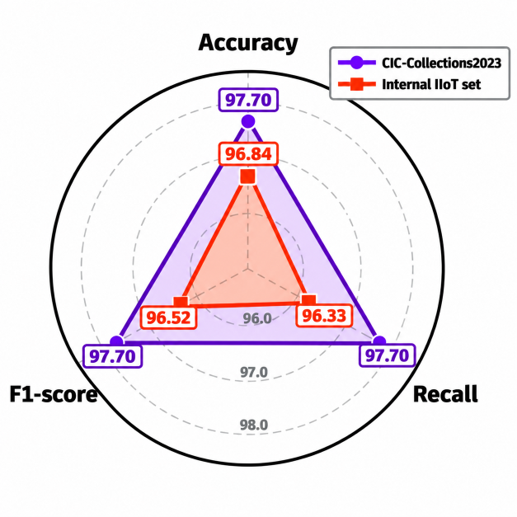
\includegraphics[width=0.72\textwidth]{figures/Picture22.png}
  \caption{Accuracy, recall and F1-score of the behavioural module, closely aligned across the public benchmark and the internal industrial set.}
  \label{fig:res-envelope}
\end{figure}

Thirdly, the error rates bound the two failure modes of the withdrawal mechanism directly. A false positive rate of 1.90\% and a false negative rate of 0.70\% were recorded on the dataset for which both are reported. The false positive figure governs the stability of the credential population, determining how much healthy traffic is misread as evidence against a device over an operating period, and the false negative figure governs exposure, determining the proportion of anomalous behaviour that never reaches the trust score at all. Most misclassifications corresponded to transient network bursts labelled as denial-of-service traffic, which is the benign direction for this failure to take, since a burst misread as an attack degrades a trust score recoverably while an attack misread as a burst does not.
 
Fourthly, generalisation between the public benchmark and the industrial set is visible as a shape rather than a scalar. Figure~\ref{fig:res-envelope} plots accuracy, recall, and F1 for both datasets on common axes, and the two performance envelopes remain closely aligned across all three measures. Alignment of that kind matters more in a federated setting than a single aggregate figure, because non-identically distributed clients are the condition under which a detector most readily specialises to one distribution, and a model that had done so would show divergent envelopes rather than parallel ones.
Lastly, per-class behaviour determines whether the aggregate figures can be relied upon at all, since a detector carrying its average on the dominant class supplies evidence that is systematically weakest exactly where an adversary operates. Figure~\ref{fig:res-perclass} reports per-class F1 on the public benchmark and the normalised confusion structure on NSL-KDD, the two being different quantities and not directly comparable to one another.
 \begin{figure}[!htbp]
  \centering
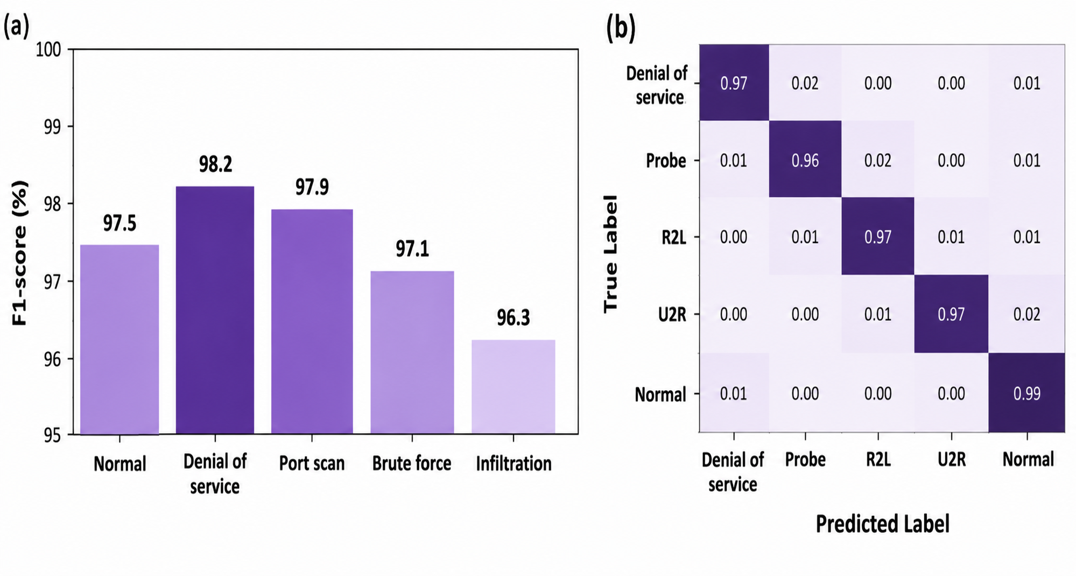
\includegraphics[width=0.98\textwidth]{figures/Picture23.png}
  \caption{Per-class F1-score on CIC-Collections2023 (a) and the normalised confusion matrix on NSL-KDD (b).}
  \label{fig:res-perclass}
\end{figure}
 

Detection capability is uniform across attack categories rather than concentrated in the dominant class. On the public benchmark the strongest class is denial of service at 98.20\% and the weakest is infiltration at 96.30\%, a spread of 1.90 percentage points. On NSL-KDD the diagonal runs from 0.99 for normal traffic to 0.96 for probe activity, a spread of 3.00 percentage points, with no class below 0.96. Infiltration and probe activity occupying the lower positions is consistent with their character, since both are low-volume categories whose traffic most closely resembles ordinary operation and both are consequently the categories a volumetric detector would miss. The off-diagonal structure confirms that the residual confusion is small and evenly distributed rather than systematic, since no off-diagonal cell exceeds 0.02 and no class loses more than four per cent of its samples in total. Withdrawal decisions therefore rest on evidence whose reliability does not depend on which attack a device is subject to.
Taken together, the aggregate figures, the error rates, the aligned envelopes, and the per-class uniformity establish that the behavioural stratum produces evidence of sufficient quality and consistency to drive a terminal decision.


\subsection{Learning Stability and the Cost of Federating}
\label{sec:eval-learning}

The behavioural module is claimed to operate inside constrained device budgets without sacrificing detection performance. The preceding subsection established what that performance is; this one establishes what it cost to obtain it under the arrangement the architecture imposes. Two costs are at issue. Distributing optimisation across clients that observe different traffic may yield a weaker global model than training on pooled data would, and a model may reach an acceptable final score by a path unstable enough that the score would not survive a different division of the data. Neither cost is visible in a final accuracy figure, so both are examined directly. The values in Table~\ref{tab:res-rounds} set the federated configuration against a centralised control trained on the same data at sampled communication rounds.

\begin{table}[!htbp]
  \centering
  \footnotesize
  \setlength{\tabcolsep}{5pt}
  \renewcommand{\arraystretch}{1.3}
  \caption{Federated and centralised configurations compared at sampled communication rounds.}
  \label{tab:res-rounds}
  \begin{tabularx}{\textwidth}{@{}
      >{\raggedright\arraybackslash}p{2.2cm}
      >{\raggedright\arraybackslash}X
      >{\raggedright\arraybackslash}X
      >{\raggedright\arraybackslash}X
      >{\raggedright\arraybackslash}X@{}}
    \toprule
    \textbf{Round} & \textbf{Centralised $F_1$} & \textbf{Centralised $\mathcal{L}$} & \textbf{Federated $F_1$} & \textbf{Federated $\mathcal{L}$} \\
    \midrule
    1  & 0.026 & 1.945 & 0.026 & 1.950 \\
    5  & 0.791 & 1.060 & 0.790 & 1.070 \\
    10 & 0.965 & 0.119 & 0.964 & 0.121 \\
    15 & 0.961 & 0.133 & 0.961 & 0.114 \\
    20 & 0.981 & 0.086 & 0.978 & 0.088 \\
    \bottomrule
  \end{tabularx}
\end{table}

The penalty for distributing optimisation is 0.003 in F1 at the twentieth round, 0.978 against 0.981, and it never exceeds that figure at any sampled point. Cost differs by no more than 0.019 across the same rounds. A margin of three thousandths is smaller than the fold-to-fold variation reported later in this subsection, which places it below the resolution at which the two configurations can be meaningfully separated. The architecture places scoring at the edge to keep traffic on the device that generated it and to stay inside the memory budget of that device; had federating cost several points of F1, those reasons would have to be weighed against a materially weaker detector. They do not.

Optimisation is front-loaded. Between the first and fifth rounds F1 rises by 0.764 and cost falls by 0.880, accounting for the greater part of the total movement in both, and the curves flatten by approximately the eighth round, after which the remaining schedule contributes little. A deployment constrained in communication rather than computation can therefore obtain most of the available performance from a short training schedule, which matters because each round costs 167~kB per client on the uplink.

One round runs against the trend and is worth examining rather than averaging away. At the fifteenth round the centralised control loses ground, its F1 falling from 0.965 to 0.961 and its cost rising from 0.119 to 0.133, while the federated configuration eases only from 0.964 to 0.961 in F1 and continues to reduce cost from 0.121 to 0.114. At the single point where the two diverge, the distributed arrangement is the steadier of the two. Averaging updates drawn from clients observing different traffic evidently damps the variance a single optimiser exhibits rather than amplifying it, which is the opposite of the behaviour usually anticipated when data is not identically distributed. Figure~\ref{fig:res-convergence} shows all four detection measures across the full schedule.

\begin{figure}[!htbp]
  \centering
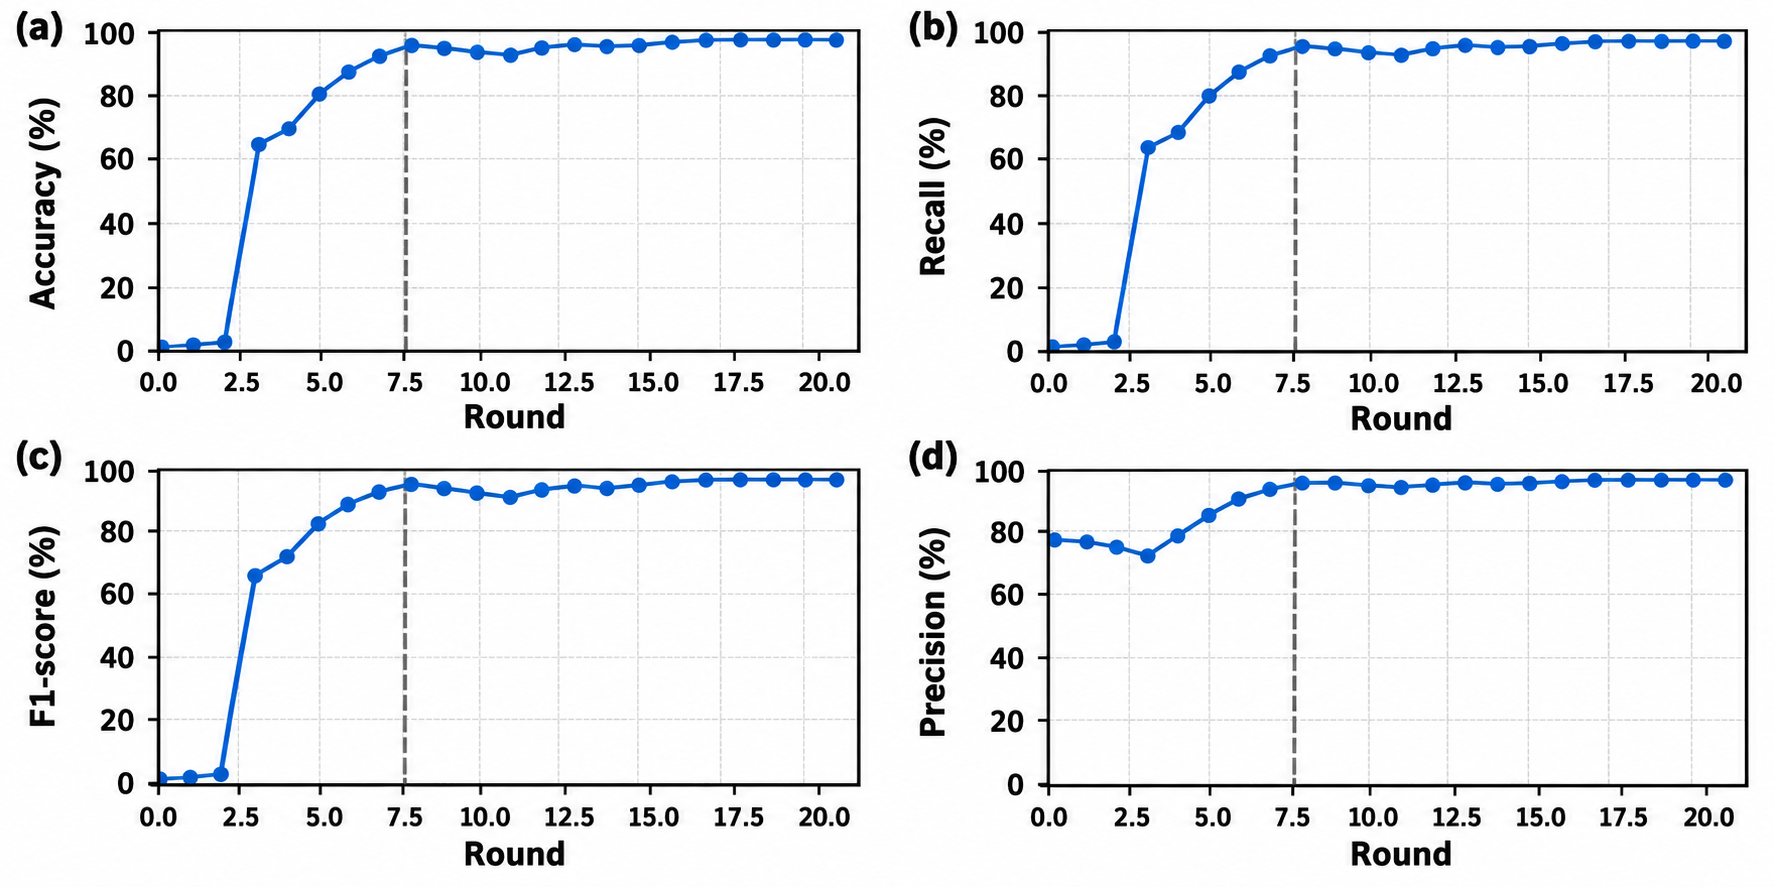
\includegraphics[width=\textwidth]{figures/Fig5_convergence_author.png}
  \caption{Convergence of accuracy (a), recall (b), F1-score (c) and precision (d) across twenty federated communication rounds on CIC-Collections2023.}
  \label{fig:res-convergence}
\end{figure}

Precision behaves unlike the other three measures from the very first round, and the difference carries operational weight. Accuracy, recall and F1 all begin near zero and climb steeply from the third round, whereas precision opens at approximately 76\% and never falls below 72\%. The model is therefore reluctant to flag healthy traffic from the outset, before it has learned to recognise anomalous traffic at all, and it acquires that recognition without becoming indiscriminate. For a mechanism that withdraws credentials terminally, this ordering is the favourable one. A model exhibiting the reverse profile, flagging readily at the start and learning restraint later, would pass through an interval during which it withdrew credentials from devices that had done nothing wrong, and no subsequent improvement would repair that. Recall and F1 track accuracy throughout the schedule, so the reduction in missed anomalies is not obtained by degrading the balance between the two error types.

Convergence on the internally generated industrial set is examined separately. That set is smaller, synthetic, and built to a different generation process, so agreement in final scores does not by itself establish that the model reached them by a comparable route. Figure~\ref{fig:res-internal} shows the progression there, plotted against training epochs rather than the communication rounds used above, since convergence on that set was tracked at the level of the local optimiser. The three measures rise together from approximately 85\% and settle at 96.84\%, 96.33\% and 96.52\% by roughly the thirtieth epoch, without oscillation, crossing, or late drift. The ordering holds throughout, with accuracy above F1 and F1 above recall at every point, so the three measures improve in concert rather than trading against one another.


\begin{figure}[!htbp]
  \centering
  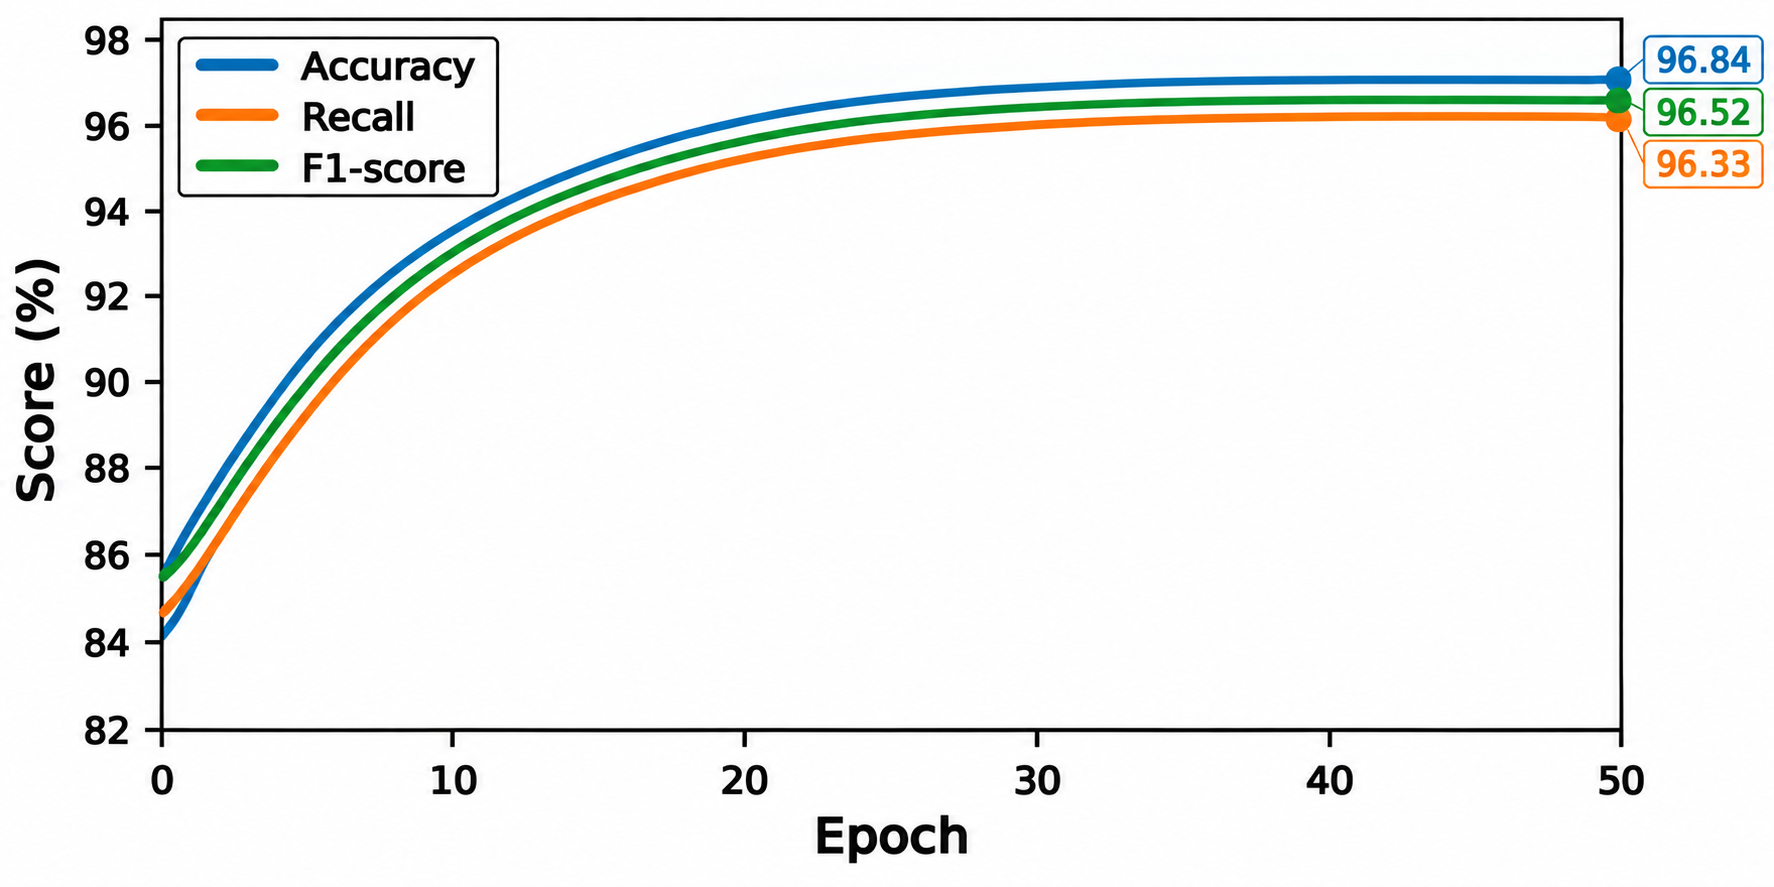
\includegraphics[width=0.80\textwidth]{figures/Fig5_internal_convergence_author.png}
  \caption{Convergence of accuracy, recall and F1-score of the behavioural module across training epochs on the internal IIoT dataset.}
  \label{fig:res-internal}
\end{figure}

The second cost concerns reproducibility rather than magnitude. A model may converge smoothly on one division of the data and differently on another, and a trust score computed from such a model would inherit that dependence. Five-fold cross-validation on both datasets tests it, and the values in Table~\ref{tab:res-cv} summarise the result.

\begin{table}[!htbp]
  \centering
  \footnotesize
  \setlength{\tabcolsep}{5pt}
  \renewcommand{\arraystretch}{1.3}
  \caption{Five-fold cross-validation on the public benchmark and the internal industrial set.}
  \label{tab:res-cv}
  \begin{tabularx}{\textwidth}{@{}
      >{\raggedright\arraybackslash}p{5.0cm}
      >{\raggedright\arraybackslash}X
      >{\raggedright\arraybackslash}X@{}}
    \toprule
    \textbf{Measure} & \textbf{CIC-Collections2023} & \textbf{Internal IIoT set} \\
    \midrule
    Mean accuracy & 97.65\% & 96.52\% \\
    Standard deviation & 0.31\% & 0.38\% \\
    Mean F1-score & 97.58\% & 96.41\% \\
    \bottomrule
  \end{tabularx}
\end{table}

Variation across folds stays below 0.40\% on both datasets, at 0.31\% on the public benchmark and 0.38\% on the industrial set, and the cross-validated means fall within 0.32 percentage points of the single-split results, at 97.65\% against 97.70\% and 96.52\% against 96.84\%. Dividing the data five ways therefore moves the outcome by less than the gap between the two datasets themselves, and the intervals drawn in Figure~\ref{fig:res-cv} are correspondingly narrow. The relevance to the architecture is specific rather than general: a trust score is accumulated from repeated evaluations, so a detector whose output shifted with the partition would produce withdrawals that reflected the training split as much as the behaviour of the device, and no threshold could be set against such a score with confidence.

\begin{figure}[!htbp]
  \centering
  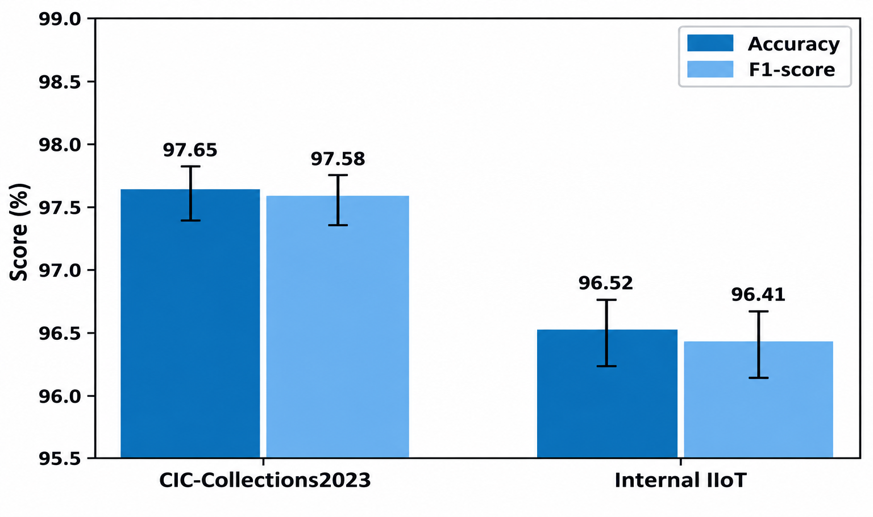
\includegraphics[width=\textwidth]{figures/Picture26.png}
  \caption{Five-fold cross-validated accuracy and F1-score on CIC-Collections2023 and the internal IIoT dataset. Error bars show one standard deviation of accuracy across folds.}
  \label{fig:res-cv}
\end{figure}

Stability on the second instantiation was established by a different method, which matters because agreement between two methods is stronger evidence than repetition of one. There the detector was trained centrally on an eighty-twenty stratified split and evaluated across five independent runs under identical conditions, with deviation across runs held under five per cent and the reported accuracy and F1 taken as means rather than best cases. Partitioning tests whether a result survives a different division of the data; repetition tests whether it survives a different initialisation of the same division. The first instantiation passes the former and the second passes the latter, and neither exposes a dependence that would undermine a score accumulated over time.

The two costs the architecture might have incurred by distributing behavioural scoring are therefore both small and both measured. Federating costs at most 0.003 in F1 against pooled training, and the result varies by under 0.40\% across partitions of either dataset. Detection performance is consequently not sacrificed by the placement decision, which settles the second half of the question this module was built to answer; whether the model that delivers it fits the compute, memory, and energy budgets of the device it runs on is settled separately by the resource analysis that follows.

\subsection{Lightweight Resource Utilisation and Deployment Feasibility}
\label{sec:eval-resource}

The two preceding subsections establish that behavioural scoring produces dependable evidence and that distributing it costs almost nothing in quality. Neither addresses the harder half of the question, which is whether the model producing that evidence can run on the device the architecture assigns it to. The distinction matters because the two failure modes are not alike. A detector that scores poorly is a weak component in a sound architecture; a detector that does not fit is a refutation of the placement decision itself, since behavioural evaluation would have to be relocated to a gateway or a server and the case for keeping traffic on the device that generated it would collapse with it. Feasibility is therefore assessed against the four budgets an industrial node actually holds, namely storage, time, processor occupancy, and energy, together with the uplink the federated arrangement consumes.

Table~\ref{tab:res-budget} sets each measured quantity against the constraint it must satisfy.

\begin{table}[!htbp]
  \centering
  \footnotesize
  \setlength{\tabcolsep}{5pt}
  \renewcommand{\arraystretch}{1.3}
  \caption{Measured resource demand of the behavioural module against the budget each quantity is constrained by.}
  \label{tab:res-budget}
  \begin{tabularx}{\textwidth}{@{}
      >{\raggedright\arraybackslash}p{4.4cm}
      >{\raggedright\arraybackslash}p{3.0cm}
      >{\raggedright\arraybackslash}X@{}}
    \toprule
    \textbf{Quantity} & \textbf{Measured} & \textbf{Constraint it sits against} \\
    \midrule
    Trainable parameters & 41{,}762 & Flash and working memory of microcontroller-class nodes \\
    Model storage under single-precision encoding & 0.17~MB & Typical 1 to 2~MB device memory budget \\
    Peak memory including activation buffers & Below 0.6~MB & The same budget, under inference load rather than at rest \\
    Inference latency & 3.1~ms per sample & Timing of the control loop the device participates in \\
    Processor occupancy at 50 inferences per second & 6 to 9\% & Headroom required by the measurement and actuation duties of the node \\
    Energy per prediction & 0.42~mJ & Power budget of a battery or harvested supply \\
    Federated update payload per round & 167~kB per client & Uplink capacity of low-rate industrial links \\
    Ledger metadata per round & 180 to 220~bytes & The same uplink, shared with the learning traffic \\
    \bottomrule
  \end{tabularx}
\end{table}

Peak memory is the decisive figure among these, and it is decisive in a way the others are not. Storage of 0.17~MB at rest rises to below 0.6~MB once activation buffers are allocated during inference, against a device budget of one to two megabytes, so the model occupies at most three fifths of the smaller budget and leaves the remainder to the application the node was installed to run. Latency and occupancy admit degradation, since a slower device can score less frequently and still function, but memory does not: a model exceeding the available allocation cannot be loaded at any inference rate, which makes this the quantity on which the placement decision stands or falls.

Processor occupancy between 6\% and 9\% at fifty inferences per second is the second constraint worth emphasising, because it is the one an industrial engineer will ask about first. A node whose primary duty is measurement and actuation cannot surrender its processor to a security function, and an occupancy figure in single digits leaves the schedule essentially intact. Energy at 0.42~mJ per prediction bears on a different deployment class, namely nodes drawing on battery or harvested supply, for which the relevant question is operating life rather than schedulability.

The ledger contributes almost nothing to the uplink it shares with the learning traffic, and Figure~\ref{fig:res-uplink} shows the proportion directly. Each round carries a model update of approximately 167~kB per client, to which the ledger adds between 180 and 220 bytes of commitment metadata. At a single client that metadata is 0.132\% of the round; at ten clients it is 0.013\%, and the per-round uplink requirement remains below 1.7~MB, within the capacity of low-power wide-area, wireless local, and industrial Ethernet links alike. The share falls as clients are added because the commitment is made once per round rather than once per client, so the ledger overhead is amortised across the federation rather than multiplied by it, and a larger deployment pays proportionally less for participation than a smaller one.

This proportion is the correct one for the architecture. The ledger exists to commit evidence about behaviour, and an arrangement in which commitment consumed a material share of the link carrying that behaviour would have inverted the relationship between the two. The on-chain validation accompanying each commitment consumes 65{,}618 gas and completes in approximately 0.11~s, so the computational cost of committing evidence is borne by the permissioned layer rather than by the device.
\begin{figure}[!htbp]
  \centering
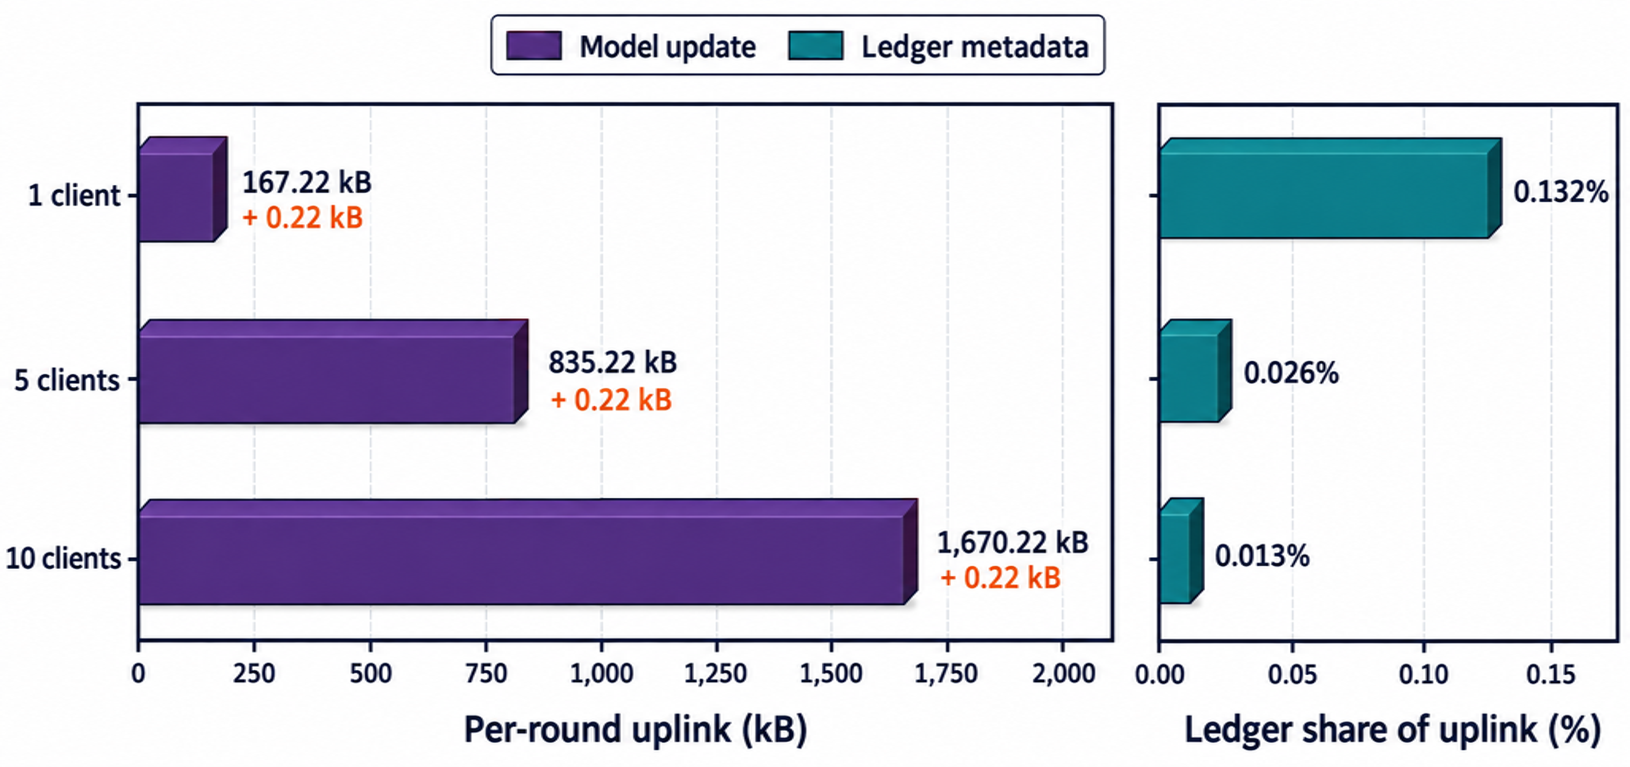
\includegraphics[width=\textwidth]{figures/Picture28.png}
  \caption{Per-round uplink composition at one, five and ten participating clients, split between the federated model update and the ledger commitment metadata, with the ledger share shown separately.}
  \label{fig:res-uplink}
\end{figure}
Whether these figures are favourable in absolute terms is established by comparison. Table~\ref{tab:res-overhead} sets the behavioural module against architectures reported in comparable federated ledger-backed detection work.
\begin{table}[!htbp]
  \centering
  \footnotesize
  \setlength{\tabcolsep}{4pt}
  \renewcommand{\arraystretch}{1.3}
  \caption{Resource profile of the behavioural module against architectures reported in comparable federated ledger-backed detection work.}
  \label{tab:res-overhead}
  \begin{tabularx}{\textwidth}{@{}
      >{\raggedright\arraybackslash}p{3.1cm}
      >{\raggedright\arraybackslash}p{1.7cm}
      >{\raggedright\arraybackslash}p{1.4cm}
      >{\raggedright\arraybackslash}p{1.4cm}
      >{\raggedright\arraybackslash}p{1.4cm}
      >{\raggedright\arraybackslash}p{1.3cm}
      >{\raggedright\arraybackslash}X@{}}
    \toprule
    \textbf{Architecture} & \textbf{Parameters} & \textbf{$M_f$ (MB)} & \textbf{$T_{inf}$ (ms)} & \textbf{$E_{inf}$ (mJ)} & \textbf{$C_{ov}$ (kB)} & \textbf{Suitability} \\
    \midrule
    Generative adversarial detector~\cite{enhanced} & 8.7\,M & 10.5 & 22.7 & 4.5 & 812 & High overhead \\
    EfficientNet-B0~\cite{FLBC-IDS} & 4.0\,M & 5.3 & 18.4 & 3.1 & 560 & High overhead \\
    Capsule autoencoder~\cite{Anitha2} & 1.2\,M & 1.8 & 11.2 & 1.9 & 240 & Medium \\
    Convolutional and multilayer hybrid~\cite{Metaverse} & 620\,k & 0.9 & 9.5 & 1.2 & 180 & Medium \\
    Behavioural module & 41{,}762 & 0.17 & 3.1 & 0.42 & 167 & Lightweight \\
    \bottomrule
  \end{tabularx}
\end{table}

The behavioural module is the least demanding architecture in the comparison on every column. Against the capsule autoencoder it carries roughly one twenty-ninth of the parameters, and against the generative adversarial detector roughly one two-hundredth. Inference is between three and seven times faster than the four comparators, at 3.1~ms against a range of 9.5 to 22.7~ms. Energy per prediction is between three and eleven times lower, at 0.42~mJ against 1.2 to 4.5~mJ. The update payload is the one column where the margin is slight, at 167~kB against 180~kB for the nearest comparator, which is expected since payload size follows parameter count only loosely once encoding overheads are included.

The column that decides feasibility, however, is memory, and there the comparison is not a matter of degree. Only the behavioural module and the convolutional hybrid fall inside a one to two megabyte allocation at rest, and once activation buffers are accounted for the margin narrows further. The capsule autoencoder at 1.8~MB consumes the entire budget before inference begins; the two largest comparators exceed it several times over. An architecture built on any of the three cannot place scoring on a microcontroller-class node at all, and must therefore site behavioural evaluation at a gateway or in the cloud. Figure~\ref{fig:res-feasibility} plots the comparison against the budget directly.


\begin{figure}[!htbp]
  \centering
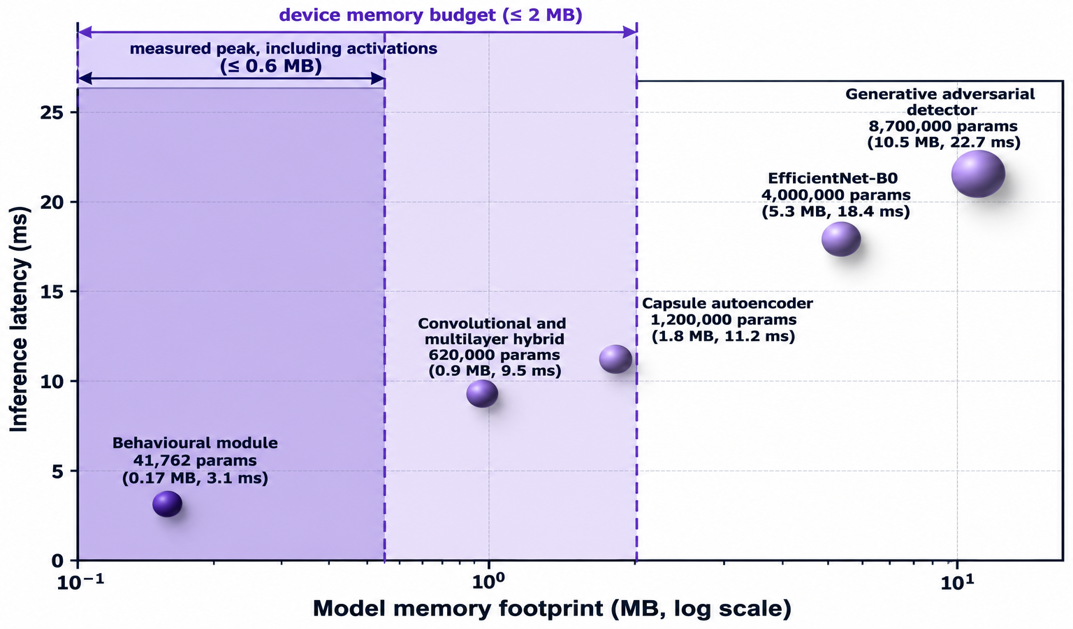
\includegraphics[width=\textwidth]{figures/Picture27.png}
  \caption{Memory footprint against inference latency for the behavioural module and four comparator architectures, with marker area proportional to parameter count and the device memory budget shaded.}
  \label{fig:res-feasibility}
\end{figure}

Two qualifications belong with these figures and are better stated here than discovered later. The energy value is an estimate obtained from an embedded-power model of a low-power microcontroller~\cite{amadi2026lightweight}, rather than a measurement taken from an instrumented device, and it should be read as an order-of-magnitude indication for the comparison rather than as a device-specific value. The latency and occupancy figures were obtained on an ARM Cortex-A53 class environment, which sits at the capable end of the constrained spectrum; a microcontroller-class part with a lower clock would be slower in proportion, though the memory figures that decide feasibility would be unchanged, since they follow from parameter count and encoding rather than from processor speed.

The resource evidence therefore settles the half of the question the two preceding subsections left open. Behavioural scoring fits within the compute, memory, and energy budgets of constrained industrial hardware, with the binding constraint satisfied at under three fifths of the smaller budget, and the ledger participation the architecture requires adds under two tenths of one per cent to the link the device already uses. Taken with the detection results, the module operates inside real device budgets without sacrificing detection performance, which is what the behavioural stratum was required to demonstrate.

\subsection{Efficient Permissioned Finalisation and Ledger Economy}
\label{sec:eval-ledger}

Behavioural evidence acquires standing only once it has been ordered and committed, and the layer performing that commitment sits directly in the path between detection and response. Two properties therefore decide whether the partition is workable in an industrial setting. Commitment must complete inside the interval within which the plant can still act on what was detected, since evidence finalised after the moment for response has passed is a record rather than a control input. And the cost of committing must remain proportionate to the frequency at which behavioural evidence arrives, because the fast layer receives a verdict for every observation window and every device, and a per-commitment cost that is merely acceptable in isolation becomes prohibitive when multiplied by that traffic. The measurements in this subsection address both, together with the consensus characteristics from which they follow.

Table~\ref{tab:led-functions} reports the cost of each contract operation carrying the write path.

\begin{table}[!htbp]
  \centering
  \footnotesize
  \setlength{\tabcolsep}{5pt}
  \renewcommand{\arraystretch}{1.3}
  \caption{Contract operations carrying the write and read paths on the permissioned instantiation, with the cost of each.}
  \label{tab:led-functions}
  \begin{tabularx}{\textwidth}{@{}
      >{\raggedright\arraybackslash}p{3.2cm}
      >{\raggedright\arraybackslash}p{2.4cm}
      >{\raggedright\arraybackslash}p{2.0cm}
      >{\raggedright\arraybackslash}X@{}}
    \toprule
    \textbf{Operation} & \textbf{Transaction cost} & \textbf{Gas} & \textbf{Role in the architecture} \\
    \midrule
    Model commitment & 64{,}778 & 65{,}618 & Commits a validated behavioural update to the permissioned layer; recurs once per observation window \\
    Server registration & 45{,}258 & 45{,}638 & Admits an aggregation server to the consortium; once per server \\
    Model retrieval & Nil & Nil & Read path used by verification and audit; unbounded in frequency \\
    \bottomrule
  \end{tabularx}
\end{table}

Commitment of a validated update consumes 65{,}618 gas and completes in approximately 0.11~s. That interval is the figure on which the partition depends, and its significance lies in what it excludes as much as in its magnitude. Because authority is assigned rather than contested, a block is final at the moment it is committed, so the 0.11~s constitutes the entire delay rather than the first instalment of one. A probabilistic mechanism reaching the same nominal interval would additionally require a confirmation depth before the record could be relied upon, and the accumulated wait would place commitment outside the window within which a supervisory loop can still act. A device flagged by the behavioural stratum can therefore be acted upon within the same cycle in which it was flagged.

The two write operations differ in how their frequency scales, and the final column of the table records that difference because it governs which cost matters. Model commitment recurs once per observation window for every participating client, so it dominates the operating cost of the layer. Server registration at 45{,}638 gas occurs once per aggregation server and is a deployment cost rather than an operating one. Retrieval costs nothing at all, and that asymmetry is deliberate rather than incidental. Verification is the operation an auditor performs, potentially frequently and potentially without any relationship to the consortium whose conduct is under examination. A design charging for reads would impose a toll on precisely the party whose scrutiny the anchoring stratum exists to invite, and would make the cost of auditing rise with the thoroughness of the audit. Writes are paid for by the operator who benefits from them; reads are free to whoever wishes to check.

Whether these costs are favourable relative to alternatives is established by comparison against public networks executing equivalent operations. Figure~\ref{fig:led-gas} reports gas consumed across the permissioned network and two public networks for three admission and commitment operations. The set compared is not identical to the set tabulated above: model commitment appears in both, while central-server registration and device registration are exercised only in the cross-network comparison and retrieval, costing nothing, is omitted from it. The central-server registration in the figure, at about 51{,}000 gas, is the value reported in the cross-network comparison of the published realisation~\cite{amadi2026lightweight} and differs from the 45{,}638 gas recorded for server registration in Table~\ref{tab:led-functions}, which comes from the deployment cost measurement of the same work. The figure is therefore read for the direction of the difference between networks rather than against the table.


\begin{figure}[!htbp]
  \centering
  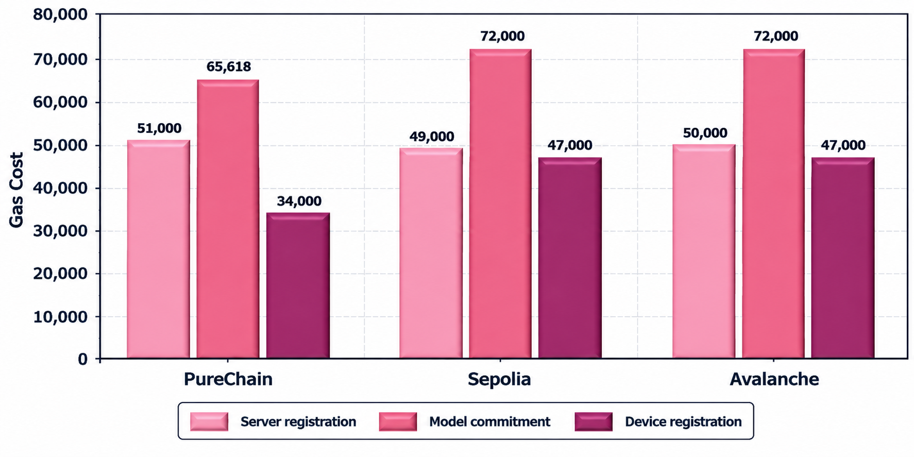
\includegraphics[width=\textwidth]{figures/Picture30.png}
  \caption{Gas consumed by the contract operations on the permissioned network and on two public networks.}
  \label{fig:led-gas}
\end{figure}

The permissioned network consumes less gas than either public network on two of the three operations compared. Model commitment costs 65{,}618 against approximately 72{,}000 on both public networks, and device registration approximately 34{,}000 against approximately 47{,}000, while central-server registration is slightly higher at roughly 51{,}000 against 49{,}000 and 50{,}000. The margin is therefore widest on device registration, and that ordering matters more than the aggregate saving. Device registration is performed once per device, so a plant that doubles its instrumented population doubles its expenditure on that operation, whereas server registration occurs once for the consortium regardless of size. The operation on which the partition saves most is the one whose total grows with the installation, and the operation on which it saves least is the one performed only at commissioning. The comparison establishes direction rather than deployment cost, since gas measures computational work and the fee attaching to it depends on the network and the moment, but the direction is the property the partition requires: high-frequency operations must be affordable on the layer to which they are assigned.
The characteristics producing these costs are those of the consensus mechanism itself. Figure~\ref{fig:led-consensus} compares it against three families in common use across the five dimensions bearing on constrained deployment.


\begin{figure}[!htbp]
  \centering
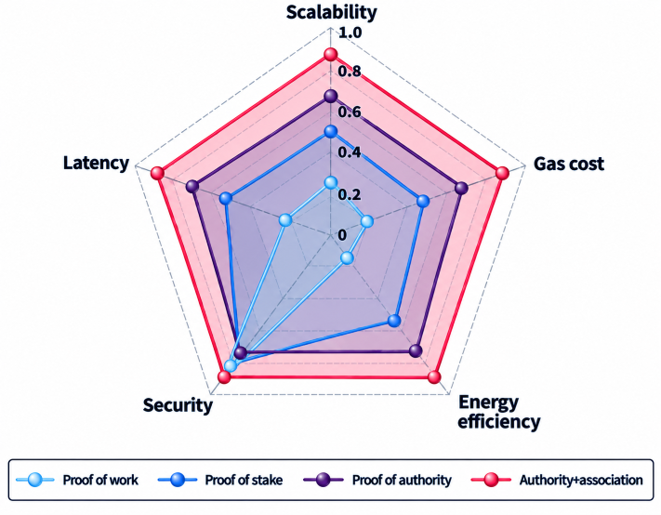
\includegraphics[width=\textwidth]{figures/Picture29.png}
  \caption{Normalised comparison of consensus mechanisms across five dimensions bearing on constrained deployment. Values are relative indicators on a unit interval rather than absolute measurements.}
  \label{fig:led-consensus}
\end{figure}

A qualification governs how this comparison may be read and is stated before the interpretation rather than after it. Only the proposed mechanism derives from direct measurement in this work. The three baselines are drawn from published experimental and simulation studies conducted under their own conditions, and all values are mapped onto a unit interval so that quantities reported in different units can be placed alongside one another. The figure therefore supports statements about relative position and supports no statement about ratios between mechanisms.

Read within that limit, the shapes rather than the individual values carry the argument. Proof of work forms a narrow spike, reaching 0.90 on security and falling to 0.15 on energy efficiency and 0.20 on gas cost, which is the profile of a mechanism that purchases assurance with expended work. The two intermediate mechanisms form progressively rounder polygons as that expenditure is reduced. The proposed mechanism encloses all three on every axis except one, and the exception is the informative part of the figure: on security it meets proof of work at 0.90 rather than exceeding it. A mechanism claiming both the lowest cost and the highest assurance would invite the suspicion that the acceptance rule had been relaxed to obtain the saving, and the figure does not make that claim.

The remainder of the profile follows from the partition rather than from the consensus mechanism alone. Scalability and latency improve together, at 0.90 on both against 0.70 and 0.75 for the nearest comparator, because high-frequency validation is separated from long-term immutable storage, so throughput does not degrade as participating devices multiply. The two properties that ordinarily trade against one another are decoupled by the partition rather than balanced within a single layer. Gas and energy efficiency improve, at 0.90 and 0.92, because authority is assigned rather than contested, which removes both proof generation and global leader election from the commitment path. The efficiency is therefore obtained by constraining who may participate, not by weakening what participation requires of them, which is why the security axis holds rather than falling.

The behaviour of the layer when its validator set is degraded completes the picture. Beyond the tolerated number of simultaneously unavailable validators, block finalisation may be delayed and new update metadata cannot be committed while the condition persists. The consequence is narrower than it appears, and it is narrower for an architectural reason rather than an incidental one. Nodes continue inference and local monitoring against the most recently verified global model, so detection is uninterrupted while commitment is stalled, and what degrades is the frequency with which the model is refreshed rather than the presence of monitoring. Integrity is preserved throughout, since unvalidated updates are rejected by access-control enforcement and by hash and dimension consistency checks and cannot reach the immutable layer. When availability is restored, aggregation and anchoring resume without rollback or loss of model consistency.

That behaviour follows directly from placing behavioural scoring below the consensus layer rather than above it. An architecture requiring consensus before a device could be evaluated would lose detection entirely under the same conditions, since no verdict could be produced until agreement was restored. Partitioning the two converts a consensus outage from a loss of coverage into a loss of freshness, and freshness is much the cheaper of the two to surrender in a plant that must continue operating while its ledger recovers.

The permissioned layer therefore satisfies both properties the partition requires of it. Commitment is final in approximately 0.11~s with no confirmation depth to wait out, which places it inside the interval within which a supervisory loop can still act; and the cost per commitment is lower than equivalent operations on public networks, with the widest margin falling on the operation whose frequency grows with the deployment. What the layer cannot supply, and was never intended to supply, is protection against the consortium that operates it, which is the responsibility of the anchoring stratum examined next.

\subsection{Verifiable Contract Security and Threat Resistance}
\label{sec:eval-security}
Performance establishes that the permissioned layer commits evidence quickly and cheaply. It establishes nothing about whether that evidence can be trusted once an adversary is assumed, and the distinction is sharper here than in most systems because the contracts carrying the write path are themselves the enforcement mechanism. A detector may be accurate, a consensus mechanism fast, and a commitment final, while a defect in the contract admits an unauthorised write that renders all three irrelevant. Assurance at this layer is therefore assessed in two ways that answer different questions: formal auditing of the contract source, which asks whether the implementation contains known classes of defect, and threat-model analysis, which asks whether the mechanisms deployed answer the capabilities an adversary is assumed to hold.

The contracts underwent static and dynamic vulnerability assessment under two complementary tools, a cloud-based formal verification platform and a static analysis framework for contract source, across six vulnerability classes. Table~\ref{tab:sec-audit} summarises the outcome.

\begin{table}[!htbp]
  \centering
  \footnotesize
  \setlength{\tabcolsep}{5pt}
  \renewcommand{\arraystretch}{1.3}
  \caption{Contract vulnerability assessment across the six classes examined.}
  \label{tab:sec-audit}
  \begin{tabularx}{\textwidth}{@{}
      >{\raggedright\arraybackslash}p{4.4cm}
      >{\raggedright\arraybackslash}p{2.4cm}
      >{\raggedright\arraybackslash}X@{}}
    \toprule
    \textbf{Vulnerability class} & \textbf{Status} & \textbf{Basis} \\
    \midrule
    Reentrancy & None found & Control-flow analysis \\
    Access control & Passed & Role checks validated \\
    Integer overflow and underflow & None found & Arithmetic safety enforced \\
    Gas inefficiencies & Minor & Optimised before deployment \\
    Timestamp manipulation & None found & Validators cross-check commit time \\
    External call risks & None found & No untrusted external calls \\
    \midrule
    Overall assessment & 98\% & Combined tool score \\
    \bottomrule
  \end{tabularx}
\end{table}

The overall figure expresses the proportion of examined classes returning no critical or high-severity finding, and its composition matters more than its magnitude. A single class was flagged, gas inefficiency, at minor severity, and it was optimised before deployment. That is the least consequential of the six for this architecture, since gas efficiency governs operating cost rather than integrity, and a contract that is expensive but sound commits the same evidence as a cheap one. The classes whose failure would have compromised the anchoring guarantee all returned clean. Reentrancy would have permitted a partially completed commitment to be re-entered and the ledger state corrupted mid-write. Arithmetic overflow would have permitted a crafted value to wrap a counter or an index and write outside its intended bounds. An unsafe external call would have handed control to code outside the audited surface during a commitment. None was found, and the absence of all three is what allows the commitment path to be treated as trustworthy in the sense the architecture requires.

Timestamp manipulation deserves separate comment, since timestamps appear in every commitment the architecture publishes and an unverifiable commit time would weaken precisely the audit trail the anchoring stratum exists to provide. The mitigation available here is one that an open network cannot offer. Validators cross-check the commit time against their own clocks, and a validator proposing an implausible timestamp is identified and attributable rather than anonymous, so the misbehaviour carries a consequence beyond rejection of the block. The residual exposure is bounded by the disagreement tolerated among validator clocks, which is a configuration parameter set by the consortium rather than an open-ended risk.

Auditing establishes that the implementation is free of known defect classes. It does not establish that the mechanisms present are sufficient against an adversary who is assumed capable rather than opportunistic, which requires the threat model. The model assumes honest but curious aggregation servers, authenticated channels, and semi-trusted validators, so an adversary is presumed able to observe legitimately and to attempt influence from within rather than merely to intrude from outside. Figure~\ref{fig:sec-threat} sets out the assets exposed under those assumptions, the capabilities attributed to an adversary, and the mechanisms deployed in response.


\begin{figure}[!htbp]
  \centering
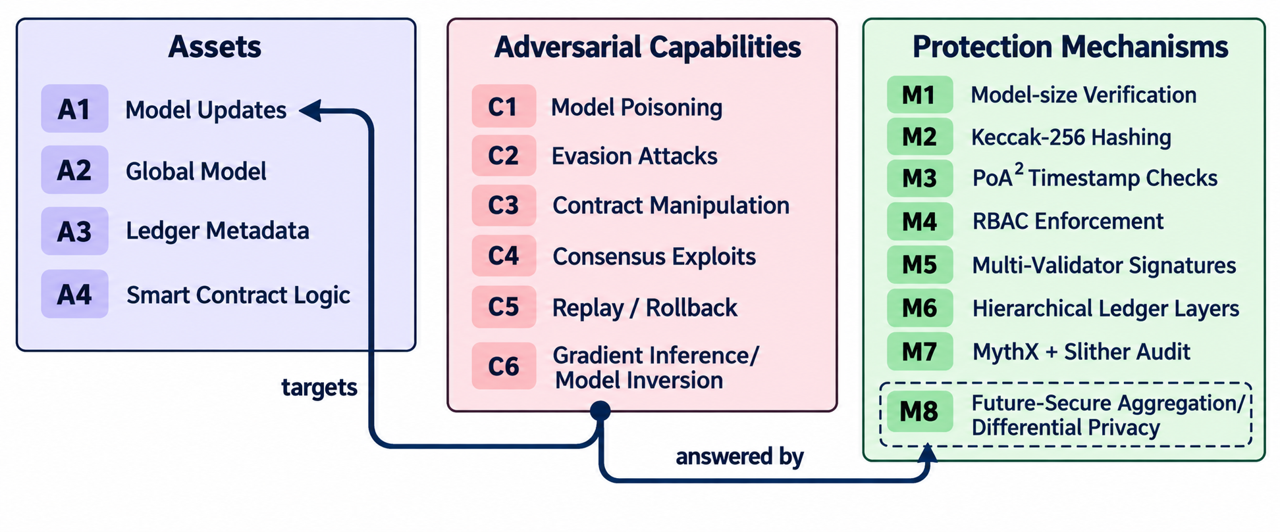
\includegraphics[width=\textwidth]{figures/Picture31.png}
  \caption{System assets, assumed adversarial capabilities, and the protection mechanisms deployed against them.}
  \label{fig:sec-threat}
\end{figure}

Most capabilities in the model are answered by a mechanism already in place. Model poisoning is met by model-size verification and dimension consistency checks, which reject an update whose shape departs from the agreed architecture before it can influence aggregation. Contract manipulation is met by role-based access control, which confines each operation to the participants entitled to invoke it. Consensus exploitation is met by multi-validator signature verification, which requires a quorum rather than a single authority. Replay and rollback are met by timestamp-based protection, which is the mechanism the audit examined separately and found sound. Ledger metadata is protected by hashing, and the layered ledger design confines the consequences of a compromise at one layer to that layer.

One capability is not answered by a deployed mechanism, and the architecture states so rather than leaving it to inference. Gradient inference and model inversion target the model updates in transit, and the present design exchanges those updates without additional cryptographic aggregation or noise injection. That choice was made deliberately, since secure aggregation and differential privacy both impose computation or accuracy costs on nodes whose budgets the preceding subsection showed to be tight, and the architecture prioritised deployability. Within the evaluated threat model the exposure is mitigated rather than eliminated: an adversary must first become an authenticated participant, updates are validated on receipt, and provenance is recorded on the ledger, so inference would have to be attempted from a position that is itself attributable. Under stronger adversarial assumptions the theoretical risk remains, and secure aggregation is designated as the mechanism answering it and identified as a priority extension rather than claimed as present.

That is the honest boundary of what this layer demonstrates. The contracts are free of the defect classes that would undermine commitment, the mechanisms deployed answer five of the six capabilities the model attributes to an adversary, and the sixth is named, its exposure bounded by the participation requirements of the consortium, and its remedy specified for future work. What no amount of contract assurance can supply is protection against the consortium itself, since every mechanism examined here is operated by the parties whose conduct an auditor may wish to examine, and it is that residual exposure the anchoring stratum exists to close.

\subsection{Optimised Quantum-Resilient Identity and Key Delivery}
\label{sec:eval-identity}
Every commitment examined so far carries a device identifier, and every exchange that produces one rests on a cryptographic assumption. Migration to post-quantum primitives is usually argued as a question of whether the replacements are secure, which they are by construction and by standardisation. On constrained hardware the question that decides deployment is different, since lattice ciphertexts and public keys are substantially larger than the elliptic-curve material they replace, and on a low-rate industrial link the bytes cost more than the arithmetic. This subsection therefore assesses fit rather than strength: whether an identifier can be derived on a field device without administrative discretion, and whether the key material protecting it can be delivered within the same budgets the behavioural module was shown to respect.

An identifier assigned administratively can be reassigned administratively, which places the operator inside the trust boundary of every claim subsequently made about the device. Deriving the identifier from entropy captured at the device removes that discretion, and Table~\ref{tab:id-comparison} sets the construction against the two alternatives available to a constrained deployment.

\begin{table}[!htbp]
  \centering
  \footnotesize
  \setlength{\tabcolsep}{5pt}
  \renewcommand{\arraystretch}{1.3}
  \caption{Identity construction compared against static and hardware-fingerprint alternatives.}
  \label{tab:id-comparison}
  \begin{tabularx}{\textwidth}{@{}
      >{\raggedright\arraybackslash}p{4.4cm}
      >{\raggedright\arraybackslash}p{2.6cm}
      >{\raggedright\arraybackslash}p{2.2cm}
      >{\raggedright\arraybackslash}X@{}}
    \toprule
    \textbf{Construction} & \textbf{Spoof resistance} & \textbf{Entropy bits} & \textbf{Adaptability} \\
    \midrule
    Address and timestamp & Low & Approximately 32 & None \\
    Hardware fingerprint with metadata & Medium & Approximately 64 & Static \\
    Entropy-seeded derivation & High & 128 and above & Real time \\
    \bottomrule
  \end{tabularx}
\end{table}

Two columns carry the argument, and they carry different halves of it. The entropy column governs whether the identifier can be published. An identifier of approximately 32 bits is enumerable, so an adversary observing the anchor could reconstruct the device population by exhaustion; at 128 bits and above it cannot, which is what permits the hashed identifier to appear on the public substrate without turning the audit record into an inventory of the plant. The adaptability column governs whether the identifier can participate in withdrawal at all. A static construction fixes what a device is and says nothing about how it behaves, so a deployment using one must maintain revocation state entirely outside the identity layer, in a register that is itself administered by the operator. A construction admitting real-time trust evolution keeps the credential and the behavioural record bound together, which is the property the withdrawal mechanism of the architecture depends upon.

Entropy quality was assessed across a thousand derived seeds of 128 bits each, with min-entropy concentrating around 0.95 and Shannon entropy falling between 0.99 and 1.0, indicating near-uniform bit distributions. The qualification stated when the plane was specified applies directly to those figures and is repeated here rather than left to the reader's memory: the sampler is software, so the measurements characterise the uniformity and reproducibility of a simulated source rather than the unpredictability a hardware generator would supply. What they do establish is that the derivation consumes and conditions its input correctly, which is the part of the construction a hardware substitution would leave unchanged, since the sample enters the digest as an opaque bit string.

Delivery of key material is where post-quantum migration is paid for on a constrained link, and Table~\ref{tab:pq-compression} reports what the delivery scheme recovers. All reductions are stated against the 768-byte Kyber512 ciphertext, which is the quantity actually transmitted.

\begin{table}[!htbp]
  \centering
  \footnotesize
  \setlength{\tabcolsep}{5pt}
  \renewcommand{\arraystretch}{1.3}
  \caption{Ciphertext size under generic and reuse-aware compression, against the 768-byte Kyber512 ciphertext.}
  \label{tab:pq-compression}
  \begin{tabularx}{\textwidth}{@{}
      >{\raggedright\arraybackslash}p{5.0cm}
      >{\raggedright\arraybackslash}X
      >{\raggedright\arraybackslash}X
      >{\raggedright\arraybackslash}X@{}}
    \toprule
    \textbf{Scheme} & \textbf{Raw size (bytes)} & \textbf{Delivered size (bytes)} & \textbf{Reduction} \\
    \midrule
    Baseline encapsulation & 768 & 768 & 0\% \\
    Generic compression & 768 & 510 & 33.6\% \\
    Reuse-aware delivery & 768 & 410 & 46.6\% \\
    \bottomrule
  \end{tabularx}
\end{table}

Generic compression recovers a third of the payload at 33.6\% and the reuse-aware scheme recovers close to half at 46.6\%, and the difference between the two is where the contribution lies rather than in the magnitude of either. Generic compression treats each ciphertext as an isolated object and must therefore compress the whole of it on every exchange. The reuse-aware scheme exploits a property of the traffic instead: successive ciphertexts to the same peer share most of their content, so the payload is fragmented, unchanged fragments are not retransmitted, and only the delta is compressed. The delivered sizes are those of the published realisation of this module~\cite{amadi2025quantum}; the reductions differ from the 36.3\% and 48.75\% reported there only because that work expressed them against the 800-byte Kyber512 public key, whereas the quantity actually transmitted, and the reference used here, is the 768-byte ciphertext.

Figure~\ref{fig:pq-delivery} shows where the difference between the two schemes comes from. Panel (a) gives the size achieved by compressing the Kyber512 ciphertext across four transmission cases, at 520, 540, 510 and 495 bytes, so generic compression alone delivers between 64\% and 71\% of the original in every case, close to the 510-byte figure of Table~\ref{tab:pq-compression}. Panel (b) gives the property the reuse-aware scheme exploits. Of the sixty-four fragments into which the ciphertext is partitioned, 51 were unchanged between transmissions and 13 changed, so most of the payload was already held by the receiver. Suppressing the retransmission of those fragments, and compressing only what changed, is what takes the delivered size from the 495 to 540 bytes of compression alone down to 410 bytes. The effectiveness of the scheme is therefore bounded by how stable the ciphertext is between sessions rather than by how compressible it is in isolation, and it retains its efficiency under mutation as the number of modified bytes rises from sixty to a hundred and twenty.


\begin{figure}[!htbp]
  \centering
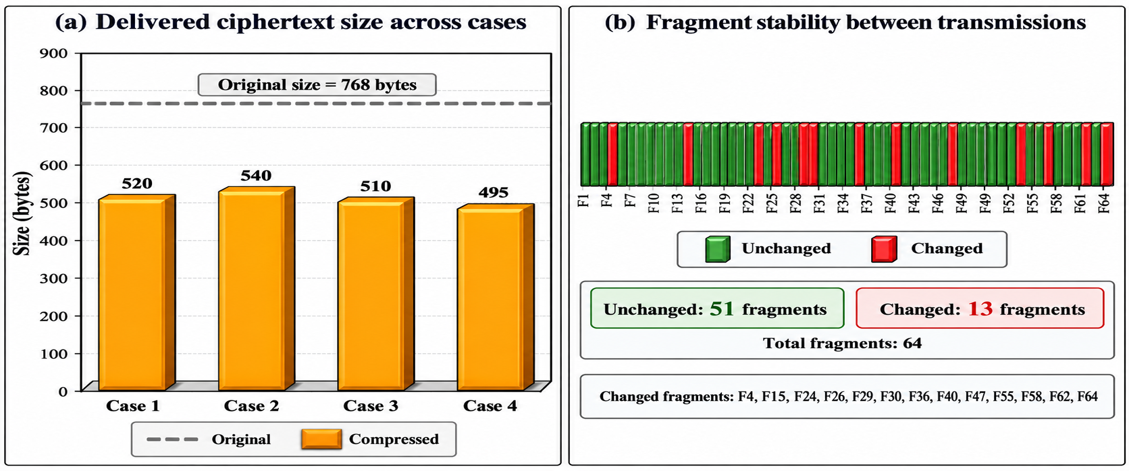
\includegraphics[width=\textwidth]{figures/Picture34.png}
  \caption{Delivered ciphertext size across simulation cases (a) and fragment stability between successive transmissions (b).}
  \label{fig:pq-delivery}
\end{figure}

The effect on the exchange itself is reported in Figure~\ref{fig:pq-latency}, and the middle bar of each panel is the instructive one.


\begin{figure}[!htbp]
  \centering
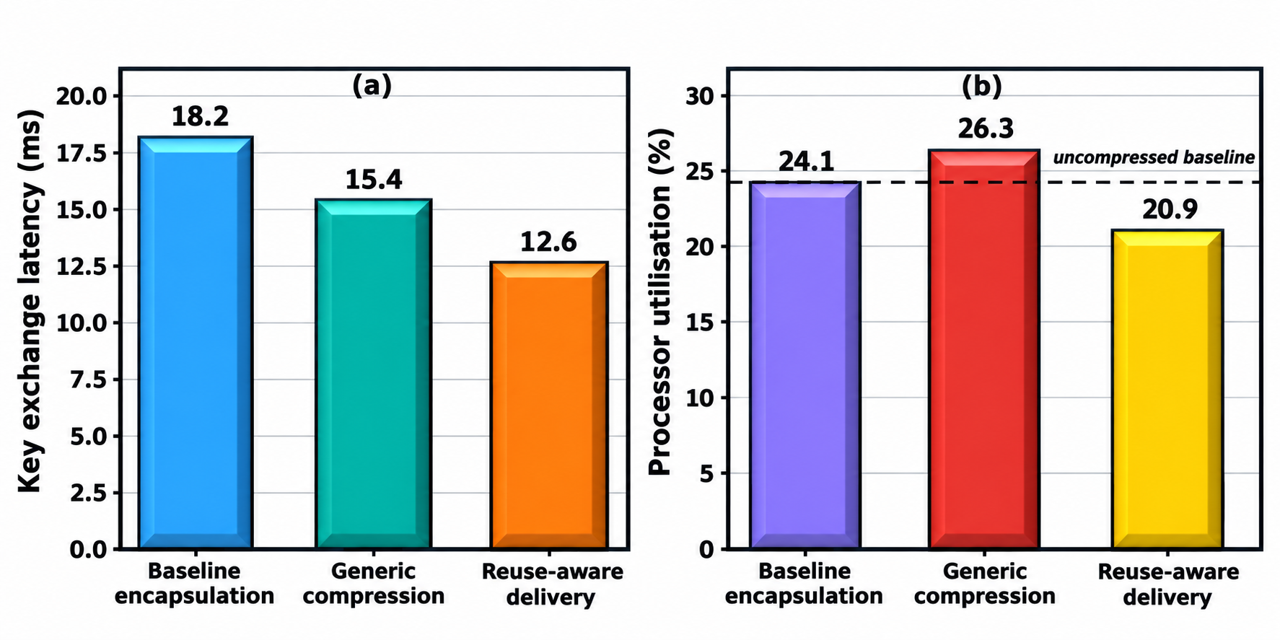
\includegraphics[width=\textwidth]{figures/Picture32.png}
  \caption{Key exchange latency (a) and processor utilisation (b) under three delivery schemes, with the uncompressed baseline marked.}
  \label{fig:pq-latency}
\end{figure}

Generic compression buys latency by spending processor time, reducing the exchange from 18.2 to 15.4~ms while raising utilisation from 24.1\% to 26.3\%, above the uncompressed baseline marked on the second panel. On a device whose primary duty is measurement and actuation that is the wrong trade, and it is the trade a deployment would unknowingly accept by applying a general-purpose compressor to post-quantum traffic. The reuse-aware scheme lowers both, reducing exchange latency by 30.7\% against the uncompressed baseline and by 18.2\% against generic compression while using less processor than either, at 20.9\%. The explanation is structural rather than incidental: fragments that are not retransmitted are also not compressed, decompressed, or reassembled, so avoiding work costs less than compressing it.

The cost of the individual primitives completes the picture, and Figure~\ref{fig:pq-operations} reports them separated by how often the architecture invokes each.
\begin{figure}[!htbp]
  \centering
  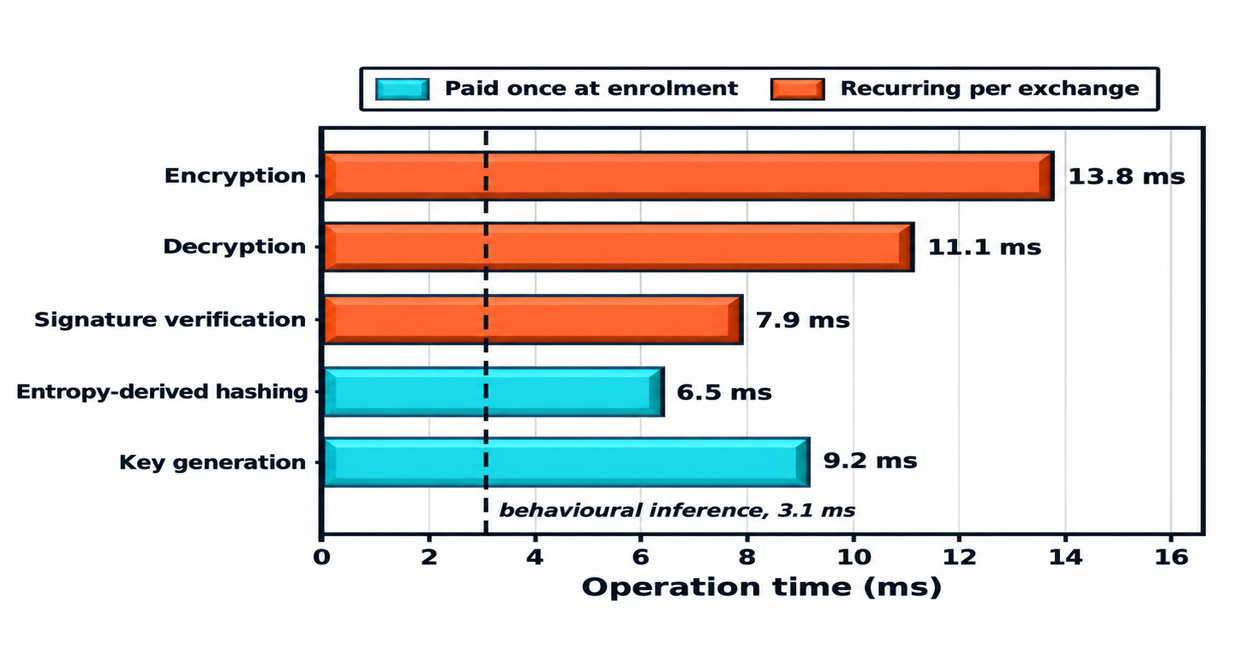
\includegraphics[width=\textwidth]{figures/Picture33.png}
  \caption{Measured cost of quantum-resilient operations on edge-class hardware, separated by enrolment and recurring use, against the behavioural inference time.}
  \label{fig:pq-operations}
\end{figure}
Enrolment operations are paid once and are irrelevant to steady-state cost, so the 9.2 and 6.5~ms attaching to key generation and hashing bear on commissioning rather than on operation. The operations that recur are encryption and decryption at 13.8 and 11.1~ms and signature verification at 7.9~ms, which together place a per-exchange cryptographic cost of 32.8~ms. Set against the 3.1~ms of behavioural inference reported earlier and marked on the figure, cryptography rather than detection is the dominant per-operation cost at the edge by a factor of roughly ten. That ordering is worth stating plainly, since it directs any future effort at reducing edge overhead toward the cryptographic path rather than toward further trimming a detector already at 41{,}762 parameters.

Selection of the primitive family followed from the same constraint rather than from a security ranking. Code-based constructions offer strong security with public keys too large for embedded nodes. Multivariate schemes have been weakened by structural attacks. Hash-based signatures are robust but impose signature sizes a low-rate link cannot absorb. The leading isogeny-based candidate, SIKE, has been broken by a classical key-recovery attack. Lattice constructions were adopted because they combine compact key material with speed adequate for constrained deployment, which is a suitability argument and is presented as one.

Two constraints bound the scope of these measurements. The compression and latency figures were obtained on a workstation-class bench, with microbenchmarks on a single-board computer, and therefore characterise the primitives rather than the microcontroller-class parts at the lower end of the device spectrum, on which the same operations would be slower in proportion to clock. Separately, the ledger bridge binding revocation to the anchoring stratum was specified but not implemented in the identity work, so the evidence reported here covers derivation, delivery, and decoding alone. The anchoring path on which those credentials depend is evidenced separately on the two ledger instantiations, and it is the binding of the two that the architecture contributes rather than either in isolation.
Post-quantum identity is therefore affordable on the hardware the architecture targets. Close to half of the ciphertext is suppressed under reuse-aware delivery, 410 of 768 bytes being sent, because the receiver already holds most of it; the exchange completes in 12.6~ms at lower processor cost than either alternative, and derivation supplies an identifier that is unenumerable when published and bound to behaviour when evaluated.


\subsection{Responsive Trust Decay and Credential Isolation}
\label{sec:eval-isolation}

Detection, commitment, and credential issue are preparatory. What the architecture ultimately does with them is withdraw a device that has begun to misbehave, and that is the operation on which its security claim finally rests. Two properties decide whether withdrawal is dependable. It must be driven by accumulated evidence rather than by a single observation, since a mechanism reacting to one detection would withdraw healthy devices on transient noise and a mechanism ignoring sustained degradation would retain compromised ones. And it must complete quickly enough that the interval during which a device known to be misbehaving still holds an honoured credential is short. The first is a property of the decay law, the second of the path between the flag and the ledger, and both are examined here together with what detection does while isolation is under way.
 
Withdrawal is governed by a trust score that falls on anomalous behaviour and recovers on normal behaviour, with two independent triggers. The score is decremented by the anomaly penalty and credited by the normal increment at each behaviour cycle, and withdrawal follows either when the score falls to the revocation threshold or when consecutive anomalous cycles exceed the streak limit. Figure~\ref{fig:iso-decay} shows the resulting trajectories for a device behaving normally and a device under sustained compromise.

\begin{figure}[!htbp]
  \centering
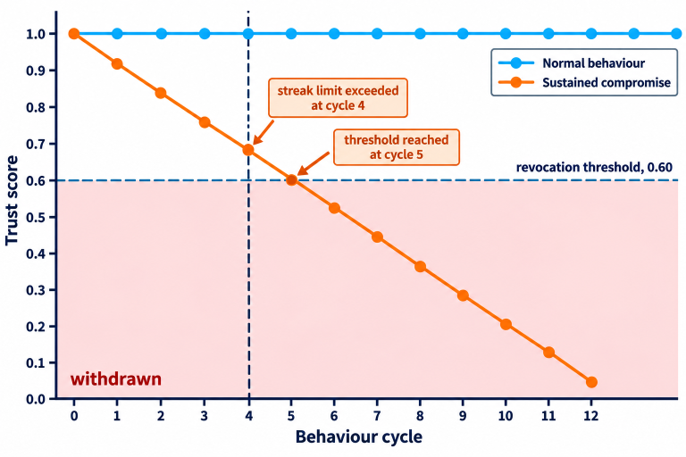
\includegraphics[width=0.98\textwidth]{figures/Picture35.png}
  \caption{Trust score evolution across behaviour cycles for a device behaving normally and a device under sustained compromise, with the revocation threshold and the withdrawn region marked.}
  \label{fig:iso-decay}
\end{figure}

The decline under sustained compromise is linear rather than exponential, which follows directly from the additive form of the law and has a consequence worth drawing out. Each anomalous cycle costs a fixed 0.08 of score, the difference between the anomaly penalty and the normal increment, so a device starting at full trust reaches the threshold of 0.60 at the fifth cycle. The number of cycles to withdrawal is therefore computable in advance from the starting score, the threshold, and the penalty, and an operator may choose the penalty to meet a required response time rather than tuning it by observation. The normal trajectory holds at its ceiling over the same interval, so a device supplying clean evidence accumulates credit rather than drifting downward, and the separation between the two widens by a fixed amount every cycle rather than depending on a single decision point.
 
The streak trigger addresses the case the threshold handles poorly, and the figure shows it firing first. A device compromised abruptly and comprehensively would, under the threshold alone, take as many cycles to withdraw as one degrading slowly, since the score falls at the same rate in both cases. Counting consecutive anomalous cycles short-circuits that delay: with a streak limit of three, a device failing every cycle in succession is withdrawn at the fourth cycle, one cycle before its score would have reached the threshold. The saving is a single cycle in this configuration and grows as the starting score rises or the penalty falls, so the two triggers answer different adversaries, gradual degradation and abrupt compromise, and the streak trigger bounds the delay that the threshold alone would leave open.
 
Elapsed time from the decision to withdraw to its confirmation on the ledger determines how long the credential remains honoured after the finding. Table~\ref{tab:iso-latency} reports that interval together with the detection quality sustained during the same runs.

\begin{table}[!htbp]
  \centering
  \footnotesize
  \setlength{\tabcolsep}{5pt}
  \renewcommand{\arraystretch}{1.3}
  \caption{Revocation latency and the detection quality sustained during isolation.}
  \label{tab:iso-latency}
  \begin{tabularx}{\textwidth}{@{}
      >{\raggedright\arraybackslash}p{5.4cm}
      >{\raggedright\arraybackslash}p{3.0cm}
      >{\raggedright\arraybackslash}X@{}}
    \toprule
    \textbf{Quantity} & \textbf{Measured} & \textbf{Basis} \\
    \midrule
    Revocation latency, flag to ledger confirmation & 1.8 $\pm$ 0.2~s & Mean over five trials \\
    Chaincode updates per revocation & Two signed updates & Per revocation event \\
    Cross-chain confirmations per revocation & One relay confirmation & Per revocation event \\
    Detection accuracy during isolation runs & 97.40\% & Same runs \\
    False positive rate & 1.90\% & Same runs \\
    False negative rate & 0.70\% & Same runs \\
    \bottomrule
  \end{tabularx}
\end{table}

Confirmation completes in 1.8~s with a spread of 0.2~s across trials, and each revocation requires two signed chaincode updates and one cross-chain relay confirmation. The narrowness of that spread matters as much as its magnitude, since a withdrawal path whose latency varied widely would leave the exposure interval unpredictable even where its mean was acceptable. The 1.8~s is measured to confirmation of the updated device status on the permissioned ledger, which is the point at which consortium participants stop honouring the credential. Publication to relying parties outside the consortium follows asynchronously through the relay, at 2.1~s between substrates under stable conditions (Table~\ref{tab:trilemma-close}), together with the confirmation depth of the public chain. The 1.8~s is also not directly comparable with the 0.11~s finalisation reported earlier, since the two were measured on different instantiations; the larger figure reflects the two signed chaincode updates each withdrawal requires on the Fabric realisation rather than a cost of the withdrawal path as such.
 
Detection quality during those runs is unchanged from the figures reported for the behavioural stratum, at 97.40\% accuracy with a false positive rate of 1.90\% and a false negative rate of 0.70\%. That invariance is the second half of what this subsection must establish, since a mechanism that isolated reliably while degrading detection would have traded one capability for another. The false positive rate bounds the cost of the mechanism in the other direction: it is the proportion of clean behaviour misread as evidence, and under an additive law those misreadings are absorbed by the normal increment across subsequent cycles rather than accumulating, so isolated false positives do not drive a healthy device toward the threshold. 
Reliability of the mechanism under load is reported in Figure~\ref{fig:iso-scale}, which gives the proportion of detected anomalies resulting in a completed withdrawal across device populations and placement strategies.

\begin{figure}[!htbp]
  \centering
  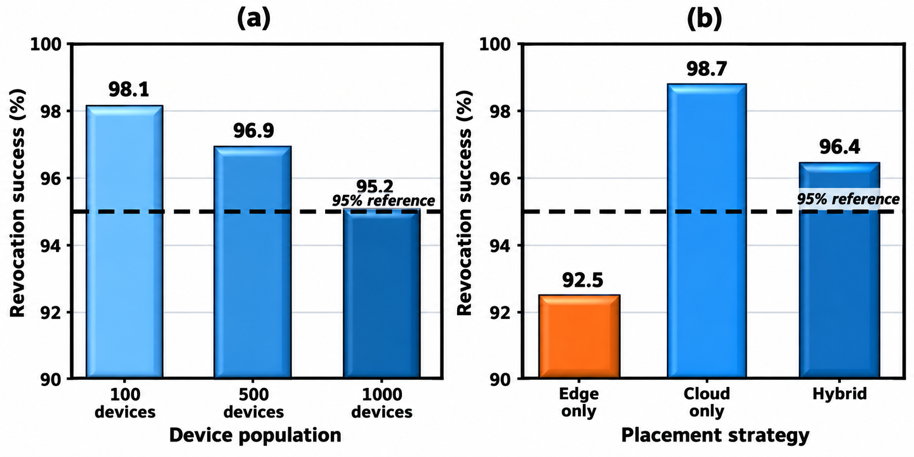
\includegraphics[width=\textwidth]{figures/Picture36.png}
  \caption{Proportion of detected anomalies resulting in a completed withdrawal, across device populations (a) and placement strategies (b).}
  \label{fig:iso-scale}
\end{figure}

Withdrawal succeeds for 98.1\% of detected anomalies at a hundred devices, 96.9\% at five hundred, and 95.2\% at a thousand. A tenfold increase in population therefore costs 2.9 percentage points of success, which is a gentle decline rather than a collapse, and it is the shape the partition predicts: the permissioned layer absorbs the growth in behavioural traffic while the withdrawal path itself is governed by the rate at which devices misbehave rather than by how many devices are present. Success remaining above 95\% at the largest population is the property that matters operationally, since a mechanism degrading sharply with scale would fail precisely in the deployments where isolation is most needed.

Placement tells a different story and exposes the one configuration that underperforms. Cloud placement achieves 98.7\% and hybrid placement 96.4\%, while edge-only placement falls to 92.5\%, below the level sustained by every permissioned configuration in the first panel. The explanation is consistent with the resource evidence presented earlier: an edge-only arrangement performs both evaluation and the assembly of the withdrawal record on the constrained device, and the same budgets that make behavioural scoring affordable there leave little headroom for the additional signing and relay work a withdrawal requires. Hybrid placement, which keeps evaluation at the edge and moves finalisation off it, recovers most of that margin at a cost of 2.3 percentage points against cloud placement, and it is the arrangement the architecture adopts.

Decay-based withdrawal therefore isolates a misbehaving device dependably and without cost to detection. The decline under sustained compromise is linear and its duration computable in advance, two triggers cover gradual and abrupt compromise respectively, confirmation reaches the ledger in 1.8~s with a spread of 0.2~s, success remains above 95\% across a tenfold increase in device population, and accuracy, false positive rate, and false negative rate are unchanged from those reported for the behavioural stratum operating without isolation under way.


\subsection{Substrate-Independent Realisation of the Partition}
\label{sec:eval-substrate}
The generality of a trust-partitioning design is a function of whether the roles it assigns can be discharged by unrelated machinery. The values in Table~\ref{tab:sub-mapping} summarise the component discharging each architectural role in the two realisations of the partition.
\begin{table}[!htbp]
  \centering
  \footnotesize
  \setlength{\tabcolsep}{5pt}
  \renewcommand{\arraystretch}{1.3}
  \caption{Architectural roles and the component discharging each in the two realisations.}
  \label{tab:sub-mapping}
  \begin{tabularx}{\textwidth}{@{}
      >{\raggedright\arraybackslash}p{3.0cm}
      >{\raggedright\arraybackslash}X
      >{\raggedright\arraybackslash}X@{}}
    \toprule
    \textbf{Role} & \textbf{Realisation I} & \textbf{Realisation II} \\
    \midrule
    Behavioural execution
      & Native fast execution layer, one record per observation window
      & Permissioned chaincode invoked per observation window \\
    Ordering and finality
      & Authority-weighted consensus, adaptive cadence, final on commit
      & Ordering service under endorsement policy, final on commit \\
    Validator identity
      & Consortium validators with authority weights and reliability tracking
      & Organisation-scoped identities from a membership service \\
    Public anchoring
      & Companion anchor receiving epoch roots, fee-free
      & General-purpose public chain, contract call, confirmation depth of three \\
    Boundary content
      & Digests and hashed identifiers only
      & Digests and hashed identifiers only \\
    \bottomrule
  \end{tabularx}
\end{table}
The data presented in Table~\ref{tab:sub-mapping} indicate that each architectural role is discharged in both realisations by components that share no consensus mechanism, no execution model, and no cost model. Four of the five rows differ entirely, spanning authority-weighted consensus against an ordering service, adaptive cadence against endorsement policy, weighted consortium validators against organisation-scoped membership identities, and fee-free anchoring against a priced public chain with a confirmation depth of three. The fifth row is identical in both, carrying digests and hashed identifiers and nothing further, which is the invariant by which the partition is defined.

The values in Table~\ref{tab:sub-properties} summarise the properties measured independently on each realisation.
\begin{table}[!htbp]
  \centering
  \footnotesize
  \setlength{\tabcolsep}{5pt}
  \renewcommand{\arraystretch}{1.3}
  \caption{Partition properties measured independently on the two realisations.}
  \label{tab:sub-properties}
  \begin{tabularx}{\textwidth}{@{}
      >{\raggedright\arraybackslash}p{4.0cm}
      >{\raggedright\arraybackslash}X
      >{\raggedright\arraybackslash}X@{}}
    \toprule
    \textbf{Property} & \textbf{Realisation I} & \textbf{Realisation II} \\
    \midrule
    Commitment finality & 0.11~s, final on commit & Final on commit, confirmation depth on the public side only \\
    Detection accuracy & 97.70\% and 96.84\% & 97.40\% \\
    Anchoring cost model & Fee-free throughout & Priced per commitment and per withdrawal \\
    Throughput under load & Sustained across the evaluated workload & 94 tx/s on Fabric with anchoring active, against 80 tx/s Fabric-only (relay experiment); 840 to 940 tx/s under the scaling workload \\
    Withdrawal confirmation & Committed on the permissioned layer & 1.8 $\pm$ 0.2~s to ledger confirmation \\
    Boundary content & Digests only & Digests only \\
    \bottomrule
  \end{tabularx}
\end{table}
The results in Table~\ref{tab:sub-properties} affirm that the properties claimed for the partition hold on both realisations. Commitment is final on commit in each, with confirmation depth arising only where the public substrate requires it. Detection accuracy spans 96.84\% to 97.70\%, a range of 0.86 percentage points across three datasets and two training regimes. Withdrawal reaches ledger confirmation in 1.8~s with a spread of 0.2~s, and the boundary carries digests alone in both cases.

Two results follow from the assignment of roles. Public-chain expenditure on the second realisation splits as the cost relation of Equation~\eqref{eq:anchor-cost} predicts, at 4.20~USD per epoch commitment against 3.50~USD per published withdrawal, assuming a gas price of 20~gwei and an ether price of 3{,}500~USD at May 2025 rates~\cite{amadi2026symmetric}. In the relay experiment, adding the anchoring layer raised Fabric throughput from 80 to 94 transactions per second, an improvement of 17.5\%, since anchoring discharges retention away from the fast layer; the 840 to 940 transactions per second of Table~\ref{tab:sota-robustness} were measured separately under the scaling workload.
The partition is therefore specifiable independently of consensus mechanism, holds under a change from fee-free to priced anchoring, is indifferent to federated or centralised training, and is satisfiable on a production enterprise stack as readily as on a purpose-built lightweight ledger. 

\section{Performance Evaluation with State-of-the-Art Approaches}
\label{sec:eval-sota}
This section evaluates the proposed architecture against recent federated blockchain intrusion detection systems and representative ledger-based data-sharing frameworks. The evaluation covers detection performance, blockchain-level cost and assurance, capability coverage across the security functions each framework provides, and robustness under varying device population and component placement.
 
\subsection{Detection Performance Against Recent Approaches}
\label{sec:sota-detection}
The results in Table~\ref{tab:sota-detection} summarise the detection performance of the proposed architecture and recent federated blockchain intrusion detection approaches, together with the model family and target system of each.
 
\begin{table}[!htbp]
  \centering
  \footnotesize
  \setlength{\tabcolsep}{4pt}
  \renewcommand{\arraystretch}{1.3}
  \caption{Detection performance of the proposed architecture against recent federated blockchain intrusion detection approaches.}
  \label{tab:sota-detection}
  \begin{tabularx}{\textwidth}{@{}
      >{\raggedright\arraybackslash}p{2.0cm}
      >{\raggedright\arraybackslash}p{0.9cm}
      >{\raggedright\arraybackslash}X
      >{\raggedright\arraybackslash}p{2.0cm}
      >{\raggedright\arraybackslash}p{1.5cm}
      >{\raggedright\arraybackslash}p{1.5cm}@{}}
    \toprule
    \textbf{Reference} & \textbf{Year} & \textbf{AI model} & \textbf{Target system} & \textbf{$A_{cc}$ (\%)} & \textbf{$R_c^{+}$ (\%)} \\
    \midrule
    \cite{Anitha2}     & 2024 & Capsule autoencoder & IIoT & 99.97 & 99.88 \\
    \cite{Metaverse}   & 2024 & CNN and MLP & Metaverse & 99.28 & n/r \\
    \cite{bfls}        & 2023 & CNN & General IoT & 98.92 & 98.90 \\
    \cite{FLBC-IDS}    & 2024 & EfficientNet and CNN & General IoT & 98.89 & 98.04 \\
    \cite{enhanced}    & 2024 & Generative adversarial & IIoT & n/r & 98.99 \\
    \cite{vehicula}    & 2021 & MLP & Vehicular IoT & 94.00 & 95.00 \\
    \cite{hbf}         & 2022 & Deep feed forward & General IoT & 90.46 & n/r \\
    \cite{BlockHunter} & 2022 & Clustering ensemble & IIoT & n/r & n/r \\
    \midrule
    Proposed (STRATA) & 2026 & CNN and LSTM & IIoT & 97.70 & 97.70 \\
    \bottomrule
  \end{tabularx}
  \vspace{2pt}
  \parbox{\linewidth}{\footnotesize n/r: not reported by the cited work.}
\end{table}
The data indicate that the proposed architecture achieves an accuracy of 97.70\% and a recall of 97.70\%, which is only slightly lower than the 99.97\% reported by the capsule autoencoder and the 99.28\% reported by the metaverse-targeted approach. The margin against the strongest entry is 2.27 percentage points. That margin is a direct consequence of model size: the capsule autoencoder carries 1.2 million parameters against the 41{,}762 of the proposed module and requires 1.8~MB of memory against 0.17~MB, so the accuracy it attains is available only at a footprint exceeding the budget of a microcontroller-class industrial node. Nevertheless, the proposed architecture exceeds the two remaining approaches that report accuracy, at 94.00\% and 90.46\%, and of the three entries targeting industrial deployment it is one of only two to report accuracy at all. It is also the only entry reporting identical accuracy and recall.
 
Secondly, in terms of balance between the two error types, the proposed architecture returns accuracy and recall at the same value while all four approaches reporting both exhibit some divergence between them, ranging from 0.02 to 1.00 percentage points. Thirdly, in terms of target system, three of the eight approaches address industrial deployment specifically, and of those the proposed architecture is the only one evaluated on industrially generated traffic in addition to a public benchmark.

\subsection{Blockchain-Level Reporting Against the Same Approaches}
\label{sec:sota-blockchain}
The results in Table~\ref{tab:sota-blockchain} highlight the blockchain-level characterisation of the proposed architecture and the same eight approaches, covering network type, transaction cost, contract assurance, and support for constrained nodes.
\begin{table}[!htbp]
  \centering
  \footnotesize
  \setlength{\tabcolsep}{4pt}
  \renewcommand{\arraystretch}{1.3}
  \caption{Blockchain-level characterisation of the proposed architecture against the same approaches.}
  \label{tab:sota-blockchain}
  \begin{tabularx}{\textwidth}{@{}
      >{\raggedright\arraybackslash}p{2.4cm}
      >{\raggedright\arraybackslash}X
      >{\raggedright\arraybackslash}p{2.0cm}
      >{\raggedright\arraybackslash}p{2.0cm}
      >{\raggedright\arraybackslash}p{2.2cm}@{}}
    \toprule
    \textbf{Reference} & \textbf{Network type} & \textbf{Gas cost} & \textbf{Security audit} & \textbf{Lightweight nodes} \\
    \midrule
    \cite{Anitha2}     & Not stated & n/r & n/r & n/r \\
    \cite{Metaverse}   & Public & 63{,}007 & No & No \\
    \cite{bfls}        & n/r & n/r & n/r & n/r \\
    \cite{FLBC-IDS}    & Permissioned & n/r & No & No \\
    \cite{enhanced}    & Permissioned & n/r & n/r & n/r \\
    \cite{vehicula}    & Public & n/r & n/r & n/r \\
    \cite{hbf}         & Permissioned & n/r & n/r & n/r \\
    \cite{BlockHunter} & Public & n/r & n/r & n/r \\
    \midrule
    Proposed (STRATA) & Hybrid & 65{,}618 & 98\% & Yes \\
    \bottomrule
  \end{tabularx}
  \vspace{2pt}
  \parbox{\linewidth}{\footnotesize n/r: not reported by the cited work.}
\end{table}
The proposed architecture consumes 65{,}618 gas for model commitment, which is only slightly higher than the 63{,}007 reported by the single approach that quantifies transaction cost. Nevertheless, that approach is the only one of eight to report any blockchain-level cost at all, none of the eight reports a contract security assessment, and none reports support for constrained nodes. All eight employ a distributed ledger and seven leave its cost unquantified, so the practical viability of those deployments remains undetermined regardless of the detection accuracy reported.
The proposed architecture reports 65{,}618 gas for commitment, a contract assessment of 98\% across six vulnerability classes, and a device profile of 41{,}762 parameters at 0.17~MB with an inference latency of 3.1~ms, and is accordingly the only entry in the comparison characterised across the artificial-intelligence layer, the blockchain layer, and the device budget simultaneously.

\subsection{Discussion of Comparative Performance}
\label{sec:sota-discussion}
Based on the presented comparative analysis, the proposed architecture achieves a detection accuracy of 97.70\% with recall at the same value, a commitment cost of 65{,}618 gas at a finalisation latency of 0.11~s, a contract assessment of 98\%, and a device footprint of 0.17~MB at 3.1~ms per inference. Approaches attaining higher raw accuracy do so with models between fifteen and roughly one hundred times larger. All but one of them exceed the memory available on microcontroller-class industrial nodes, which confines behavioural evaluation to a gateway or a server, and the one that fits at rest, at 0.9~MB, leaves little headroom once activation buffers are allocated.
Jointly optimising the detector and the ledger deployment, and characterising both against the resource constraints of industrial edge hardware, is what distinguishes the proposed architecture from approaches optimising either in isolation. The comparison therefore establishes the proposed architecture as a deployable option for industrial environments in which detection quality, ledger cost, contract assurance, and device budget must be satisfied together rather than individually.


\subsection{Comparison with Related Hybrid-Ledger Approaches}
\label{sec:sota-related}
The results in Table~\ref{tab:sota-related} highlight the capability coverage of the proposed architecture and representative ledger-based data-sharing frameworks across device lifecycle management, threat detection, quantum-resilient cryptography, public auditability, and performance reporting.
\begin{table}[!htbp]
  \centering
  \footnotesize
  \setlength{\tabcolsep}{4pt}
  \renewcommand{\arraystretch}{1.3}
  \caption{Capability coverage of the proposed architecture against representative ledger-based data-sharing frameworks.}
  \label{tab:sota-related}
  \begin{tabularx}{\textwidth}{@{}
      >{\raggedright\arraybackslash}p{2.4cm}
      >{\raggedright\arraybackslash}p{2.1cm}
      >{\centering\arraybackslash}p{0.9cm}
      >{\centering\arraybackslash}p{0.9cm}
      >{\centering\arraybackslash}p{1.2cm}
      >{\centering\arraybackslash}p{1.2cm}
      >{\raggedright\arraybackslash}X@{}}
    \toprule
    \textbf{Method} & \textbf{Chain type} & \textbf{DLM} & \textbf{ITD} & \textbf{PQC} & \textbf{Audit} & \textbf{Performance reporting} \\
    \midrule
    \cite{yangwei}    & Single & \checkmark & $\times$ & $\times$ & \checkmark & Limited, chain focus \\
    \cite{liu}        & Permissioned & \checkmark & \checkmark & $\times$ & $\times$ & Limited, case specific \\
    \cite{reshma}     & Hybrid & \checkmark & $\times$ & $\times$ & \checkmark & Partial, crypto focus \\
    \cite{wang}       & Hybrid & \checkmark & $\times$ & $\times$ & \checkmark & Partial, health domain \\
    \cite{erukala}    & Hybrid & \checkmark & $\times$ & $\times$ & \checkmark & Limited, end-to-end communication \\
    \cite{ghaemi}     & Single with QC & $\times$ & $\times$ & \checkmark & $\times$ & Partial, authentication protocol \\
    \cite{aslam}      & Single with PQC & $\times$ & $\times$ & \checkmark & \checkmark & Partial, consensus and cryptography \\
    \cite{venkatesh}  & Single with QC & $\times$ & $\times$ & \checkmark & $\times$ & Partial, lightweight claims \\
    \midrule
    Proposed (STRATA) & Hybrid & \checkmark & \checkmark & \checkmark & \checkmark & Full, learning, cryptography, ledger and robustness \\
    \bottomrule
  \end{tabularx}
  \vspace{2pt}
  \parbox{\linewidth}{\footnotesize\raggedright
  DLM-device lifecycle management; ITD-intelligent threat detection; PQC-post-quantum and quantum-resilient cryptography.}
\end{table}
It indicates that the architecture is the only entry supporting all four capabilities. Five of the eight frameworks provide device lifecycle management, one provides intelligent threat detection, three provide quantum-resilient cryptography, and five provide public auditability, with no framework supporting more than three of the four.
 
The coverage divides along a consistent line. The five frameworks providing lifecycle management and auditability rely on classical cryptography and address no quantum threat, while the three providing quantum-resilient cryptography operate on single-chain designs and provide neither lifecycle governance nor ledger-triggered revocation. Threat detection appears in one framework alone and is not coupled to revocation in that case. The proposed architecture combines lifecycle governance, hybrid-chain auditability, and learning-driven revocation within a single operational workflow, which is consistent with the latency, throughput, and revocation results reported earlier in this chapter.
Performance reporting separates the entries further. Seven of the eight frameworks report performance partially, confined to a chain, a protocol, or a domain, and one reports it in limited form. The proposed architecture reports detection quality, cryptographic overhead, ledger cost, and robustness across deployment conditions under a single experimental setting, which permits the four to be assessed jointly rather than in isolation.

\subsection{Robustness Across Deployment Conditions}
\label{sec:sota-robustness}
The values in Table~\ref{tab:sota-robustness} summarise latency, throughput, and revocation success across six deployment scenarios spanning device population and component placement.
\begin{table}[!htbp]
  \centering
  \footnotesize
  \setlength{\tabcolsep}{5pt}
  \renewcommand{\arraystretch}{1.3}
  \caption{Latency, throughput, and revocation success across six deployment scenarios, mean of five runs.}
  \label{tab:sota-robustness}
  \begin{tabularx}{\textwidth}{@{}
      >{\raggedright\arraybackslash}p{4.6cm}
      >{\raggedright\arraybackslash}X
      >{\raggedright\arraybackslash}X
      >{\raggedright\arraybackslash}X@{}}
    \toprule
    \textbf{Scenario} & \textbf{Latency (ms)} & \textbf{Throughput (tx/s)} & \textbf{Revocation success (\%)} \\
    \midrule
    100 devices & 32.4 & 910 & 98.1 \\
    500 devices & 47.8 & 885 & 96.9 \\
    1000 devices & 68.3 & 840 & 95.2 \\
    Edge-only placement & 54.2 & 740 & 92.5 \\
    Cloud-only placement & 30.7 & 940 & 98.7 \\
    Hybrid placement & 40.1 & 895 & 96.4 \\
    \bottomrule
  \end{tabularx}
\end{table}
The results affirm that the architecture scales without collapse. A tenfold increase in device population raises latency from 32.4 to 68.3~ms and reduces throughput from 910 to 840 transactions per second, a loss of 7.7\%, while revocation success remains above 95\% throughout. Latency increases gradually rather than sharply, which is consistent with leader-driven log replication under the ordering service as the participating population grows.
 
Across placement strategies, cloud placement achieves the highest throughput at 940 transactions per second and the lowest latency at 30.7~ms, and edge-only placement the lowest throughput at 740 and a revocation success of 92.5\%. Hybrid placement returns 895 transactions per second at 40.1~ms with revocation success of 96.4\%, retaining 95\% of cloud throughput while keeping behavioural evaluation on the devices generating the traffic. Revocation success exceeds 95\% in every scenario apart from edge-only placement, confirming that lifecycle enforcement and anomaly-triggered revocation sustain scale across the evaluated deployment range.

\section{Summary of Results}
\label{sec:eval-summary}

After analysing the results and discussions presented, it is possible to establish trustworthy security for constrained industrial deployments in real time by combining behavioural evidence derived from a lightweight learnable model with the finalisation, anchoring, and credential parameters carried by a partitioned hybrid ledger. Behavioural scoring at 41{,}762 parameters and 0.17~MB supplies detection between 96.84\% and 97.70\% within the compute, memory, and energy budgets of microcontroller-class hardware; authority-weighted finalisation commits that evidence in 0.11~s without confirmation depth; epoch anchoring places a compact proof of it beyond the reach of the operating consortium; and entropy-seeded credentials delivered under post-quantum encapsulation bind each verdict to a device whose identifier cannot be enumerated from the public record.

With the proposed STRATA architecture in place, there is an enhancement in the security capacity of constrained industrial deployments for continuous and verifiable monitoring, since each security function is discharged on the layer whose cost profile sustains it rather than uniformly across devices that cannot afford uniform protection. High-frequency behavioural validation is absorbed by a fast permissioned layer at 0.13\% of the link the learning traffic already occupies, while low-frequency identity anchoring, audit, and revocation are committed to a separate public layer at a cost governed by how often devices misbehave rather than by how much traffic they generate. Credential withdrawal follows accumulated evidence rather than a single detection, reaching ledger confirmation in 1.8~s and succeeding for above 95\% of detected anomalies across a tenfold increase in device population, without degradation of the detection quality on which those decisions rest.

This combined approach ensures that an industrial deployment is capable of detecting anomalous device behaviour, attributing it to an identified credential, and withdrawing that credential verifiably, while continuing to monitor throughout. Detection persists during consensus outage because behavioural scoring is placed below the consensus layer, so a validator failure costs freshness of the global model rather than coverage of the plant. Anchoring imposes no disclosure surface, since digests and hashed identifiers alone cross the trust boundary on both realisations. Contract assurance across six vulnerability classes returned no critical or high-severity finding, and the architecture is the only entry in the comparative evaluation reporting ledger cost, contract assessment, and support for constrained nodes together.

By realising this approach on two ledger substrates sharing no consensus mechanism, no execution model, and no cost model, the generality of trust-partitioning is established beyond a single implementation. Security functions are placed by cost profile rather than by uniform application, the resulting design operates within the resource limits of industrial edge hardware, and its organising principle transfers to substrates chosen for their difference.

\subsection{Answers to the Research Questions}
\label{sec:eval-rq}

Table~\ref{tab:rq-answers} draws the results of this chapter together against the five research questions posed in Section~\ref{sec:rq}, stating for each the principal evidence, the section in which it is reported, and the extent to which the question is answered. Where an answer holds only within a stated scope, the scope is recorded rather than left implicit.

\begin{table}[!htbp]
  \centering
  \footnotesize
  \setlength{\tabcolsep}{4pt}
  \renewcommand{\arraystretch}{1.3}
  \caption{Answers to the research questions, with the principal evidence and its location in this chapter.}
  \label{tab:rq-answers}
  \begin{tabularx}{\textwidth}{@{}
      >{\raggedright\arraybackslash}p{0.9cm}
      >{\raggedright\arraybackslash}X
      >{\raggedright\arraybackslash}p{2.0cm}
      >{\raggedright\arraybackslash}p{3.0cm}@{}}
    \toprule
    \textbf{RQ} & \textbf{Principal evidence} & \textbf{Reported in} & \textbf{Answer} \\
    \midrule
    RQ1 & Permissioned finalisation in 0.11~s with no confirmation depth; ledger metadata at 0.13\% of the learning uplink; public-layer cost governed by the revocation rate rather than traffic volume; anchoring raises Fabric throughput from 80 to 94~tx/s
        & Sections~\ref{sec:eval-resource}, \ref{sec:eval-ledger}, \ref{sec:eval-substrate}
        & Yes: partitioning delivers verifiable security within device and ledger budgets \\
    RQ2 & 41{,}762 parameters at 0.17~MB (peak below 0.6~MB), 3.1~ms inference, 6 to 9\% processor occupancy; accuracy 96.84 to 97.70\% across three datasets; federation costs at most 0.003 in F1
        & Sections~\ref{sec:eval-evidence} to~\ref{sec:eval-resource}
        & Yes, on edge-class hardware; energy figure estimated rather than instrumented \\
    RQ3 & Kyber512 ciphertext reduced from 768 to 410~bytes (46.6\%); key exchange 30.7\% faster at lower processor load; identifiers of 128 bits and above
        & Section~\ref{sec:eval-identity}
        & Yes, on a workstation bench with single-board microbenchmarks; ledger bridge specified but not implemented \\
    RQ4 & The same partition realised on PureChain NSL and on Fabric with Ethereum, sharing no consensus, execution, or cost model; boundary content limited to digests in both
        & Section~\ref{sec:eval-substrate}
        & Yes, on two substrate pairs; a general characterisation remains open \\
    RQ5 & Two independent withdrawal triggers; confirmation in 1.8~$\pm$~0.2~s; success of 95.2\% or more up to 1{,}000 devices; detection unchanged during isolation (97.40\%, false positive rate 1.90\%); contract assessment of 98\%
        & Sections~\ref{sec:eval-security}, \ref{sec:eval-isolation}, \ref{sec:sota-robustness}
        & Yes, within the evaluated threat model; inference attacks on model updates not mitigated \\
    \bottomrule
  \end{tabularx}
\end{table}

\subsection{Resolution of the Security, Scalability, and Speed Trilemma}
\label{sec:eval-trilemma}
The security, scalability, and speed trilemma presented at the outset of this thesis holds within a single distributed ledger, where optimising any two dimensions is obtained at the expense of the third. The values in Table~\ref{tab:trilemma-close} summarise the evidence obtained on each dimension and the layer supplying it.

\begin{table}[!htbp]
  \centering
  \footnotesize
  \setlength{\tabcolsep}{5pt}
  \renewcommand{\arraystretch}{1.3}
  \caption{Evidence obtained on each dimension of the trilemma and the layer supplying it.}
  \label{tab:trilemma-close}
  \begin{tabularx}{\textwidth}{@{}
      >{\raggedright\arraybackslash}p{2.0cm}
      >{\raggedright\arraybackslash}p{3.2cm}
      >{\raggedright\arraybackslash}X
      >{\raggedright\arraybackslash}p{2.4cm}@{}}
    \toprule
    \textbf{Dimension} & \textbf{Supplied by} & \textbf{Measured evidence} & \textbf{Cost incurred} \\
    \midrule
    Security
      & Public anchoring stratum, with contract assessment on the permissioned layer
      & No critical or high-severity finding across six vulnerability classes at an overall assessment of 98\%; integrity preserved beyond the fault bound, with unvalidated updates unable to reach the immutable layer
      & Anchoring fee per epoch and per withdrawal \\
    Speed
      & Consensus and coordination stratum
      & Finalisation in 0.11~s with no confirmation depth; behavioural inference in 3.1~ms at the edge; withdrawal confirmed in 1.8~s
      & Validator set restricted to identified participants \\
    Scalability
      & Separation of the two strata
      & Throughput of 840 to 910 transactions per second across 100 to 1000 devices, and up to 940 under cloud placement, a reduction of 7.7\% across a tenfold population increase under the scaling workload; in the relay experiment, 94 against 80 transactions per second relative to a Fabric-only baseline
      & Relay latency of 2.1~s between substrates under stable conditions \\
    \bottomrule
  \end{tabularx}
\end{table}

The data presented indicate that each dimension is discharged by a different part of the architecture and paid for in a currency the supplying layer sustains. Security rests on a substrate outside consortium administration, which incurs a transaction fee and no latency penalty, since anchoring proceeds asynchronously to the control loop it protects. Speed rests on assigned rather than contested authority, which restricts participation and returns deterministic finality at a tenth of a second. Scalability arises from the separation itself rather than from optimisation within either layer, as evidenced by the single-chain comparison in which the addition of the anchoring layer raised throughput by 17.5\% rather than lowering it.

The trilemma is therefore not resolved within a layer but dissolved across two. Once each demand is routed to the layer whose cost profile matches it, the trade-offs that bind within a single ledger become budgetary decisions distributed between substrates, and the architecture sustains all three dimensions simultaneously at the operating points reported throughout this chapter. Trust-partitioning accordingly delivers lightweight, verifiable, and quantum-resilient security for constrained mission-critical industrial deployments, which is the position the thesis set out to establish.